\documentclass[a4paper, 12pt]{book}
\usepackage{natbib}
\usepackage{url}
\usepackage{graphicx}
\usepackage{subcaption}
\usepackage{textcomp}
\usepackage{rotating}
\usepackage{multirow}
\usepackage{amsmath}
\usepackage{verbatim}
\usepackage{makecell}
\usepackage{xspace}
\usepackage[table]{xcolor}
\usepackage[T1]{fontenc}

\definecolor{yes}{rgb}{0.9,1,0.9}
\definecolor{no}{rgb}{1,0.9,0.9}
\definecolor{maybe}{rgb}{1,1,1}

\newcommand{\Wifi}{Wi-Fi\xspace}
\newcommand{\wifi}{Wi-Fi\xspace}
\newcommand{\apps}{apps\xspace}
\newcommand{\app}{app\xspace}
\newcommand{\BRP}{Blackout Resistent Positioning\xspace}
\newcommand{\aBRP}{BRP\xspace}
\newcommand{\device}{smartphone\xspace}
\newcommand{\devices}{smartphones\xspace}
\newcommand{\Device}{Smartphone\xspace}
\newcommand{\Devices}{Smartphones\xspace}
\newcommand{\mpp}{multi-path propagation\xspace}
\newcommand{\Mpp}{Multi-path propagation\xspace}
\newcommand{\mpi}{multi-path interference\xspace}
\newcommand{\mpid}{multi-path interference drop\xspace}
\newcommand{\mpids}{multi-path interference drops\xspace}
\newcommand{\Mpi}{Multi-path interference\xspace}
\newcommand{\wordcount}[1]{
    \immediate\write18{make -C #1 wordcount.tex}
    \input{#1/wordcount.tex}
}

\newcommand{\urlref}[1]{\footnote{\url{#1}}}
\newcommand{\chapterref}[1]{chapter \ref{chap:#1}}
\newcommand{\appendixref}[1]{appendix \ref{app:#1}}
\newcommand{\figureref}[2]{figure \ref{fig:#1-#2}}
\newcommand{\Figureref}[2]{Figure \ref{fig:#1-#2}}
\newcommand{\tableref}[2]{table \ref{tbl:#1-#2}}
\newcommand{\Tableref}[2]{Table \ref{tbl:#1-#2}}
\newcommand{\sectionref}[2]{section \ref{sec:#1-#2}}
\newcommand{\Sectionref}[2]{Section \ref{sec:#1-#2}}
\newcommand{\equationref}[2]{equation \ref{eq:#1-#2}}


\newcommand{\define}[1]{\begin{em}#1\end{em}}
\newcommand{\gnuplotscale}[4]{
    \immediate\write18{make -C #1 #2-gnuplot.tex}
    \scalebox{#4}{\input{#1/#2-gnuplot}}
    \caption{#3}
    \label{fig:#1-#2}
}
\newcommand{\gnuplot}[3]{
    \immediate\write18{make -C #1 #2-gnuplot.tex}
    \input{#1/#2-gnuplot}
    \caption{#3}
    \label{fig:#1-#2}
}
\newcommand{\fig}[1]{
    \begin{figure}[ht]
        #1
    \end{figure}
}

%\includeonly{rss/chapter}

\def\mySfFamily{\fontfamily{qcr}\selectfont \sffamily }
\begin{document}

\title{BLE positioning (\input{wordcount.tex})}
\author{Reinoud Elhorst}
\date{\today}
\maketitle

\chapter{Introduction}
\wordcount{introduction}

Using digital devices to find one's position has been one of the great advancements in technology in the last couple of decades, and has more recently entered the domain of personal electronics.
At the end of 2013, it was reported that more than one in five persons owns a smartphone\urlref{http://www.businessinsider.com/smartphone-and-tablet-penetration-2013-10}{8 June 2014}, and many of these smartphones include GPS (General Positioning System) receivers.
In addition, many GPS receivers have been sold outside of smartphones, in stand-alone navigation devices, or built in to larger products, such as cars.
Since in 2000 the Selective Availability of GPS ended, the accuracy has improved to within a couple of meters\urlref{http://www.gps.gov/systems/gps/modernization/sa/}{8 June 2014}.
More technological enhancements are possible to reduce the error into the centimeter range\urlref{http://en.wikipedia.org/wiki/GPS_enhancement}{8 June 2014}.
The GPS system (and similar systems such as the EU's Galileo, Russia's GLONASS, India's IRNSS and China's Beidou-2 system), collectively known as \emph{Global Navigation Satellite Systems} (GNSS), have become the standard for outdoor positioning, even though mobile and \wifi signals are also being used to enhance positioning performance by many devices.

In addition to being available globally for free, and providing accurate positioning, GNSS have some further advantages that resulted in their wide-spread adoption.
GNSS can be used without any additional information, meaning that devices without an internet connection (either because they don't support an internet connection, or they currently are not connected), can position using GNSS.
The communication from satellite to positioning device is completely one way, meaning on the one hand that the system scales perfectly with additional positioning devices, on the other hand does it guarantee perfect privacy: using a positioning device can be done without anyone finding out that a device is even being used.
Finally, GNSS have some unique security properties: even though the civilian GPS system is vulnerable to jamming and spoofing\citep{volpe2001vulnerability,grant2009gps}, countermeasures are available\citep{warner2003gps,lo2009signal}.
In addition, the physical security to the senders is large, as disabling, stealing, or tampering with a satellite is a complex and expensive operation.

The signals from GNSS satellites are weak, and usually unable to penetrate structures.
This means that the system's use degrades considerably between high-rise buildings, and cannot be used indoors.
In addition, indoor positioning is harder, because there are more variables; while outdoors one can usually assume that the positioning device is on ground level, indoors positioning needs to be done in all 3 dimensions.
Finally, indoor positioning for consumer use has stricter requirements than outdoors: while outdoors an error of 10 meters can easily be spotted and corrected for by a user, indoors 10 meters can mean a different floor, or even building. 
There has been much research into indoor positioning, e.g.\ using infra-red\citep{want1992active}, a combination of ultrasound and radio-waves\citep{harter2002anatomy,priyantha2000cricket} or radio-waves by themselves\citep{lorincz2005motetrack}.
Where GPS is not available, or in addition to GNSS positioning, current smartphones use a combination of mobile signals from cell towers, and \wifi signals, use of which was pioneered by \citet{bahl2000radar}.
The choice for these technologies is at least partly because both the beacon infrastructure and the smartphone hardware to receive the signals, was already in place.
Positioning through \wifi is accurate to tens of meters in a typical urban environment\citep{zandbergen2009accuracy}, and the precision increases with the number of access points in close vicinity.
Using mobile signals for positioning gets an accuracy in hundreds of meters.

\section{\BLE}
\BLE (BLE), also known as Bluetooth Smart, or sometimes incorrectly referred to as Bluetooth 4.0\footnote{Bluetooth 4.0 is the fourth incarnation of the Bluetooth standard, which contains, among other things, \BLE. The latest Bluetooth standard is 4.1, from 21 December 2013, which includes some big changes for \BLE as well; there changes however have no effect on packet advertising, and I do not believe that any of the changes is of influence on the technology described in this report.}, is a new wireless connection technology that is quickly gaining in popularity.
It was introduced in 2010 as part of the Bluetooth 4.0 standard.
BLE is not compatible with previous versions of Bluetooth (now often referred to as Bluetooth Classic), and is not meant to replace traditional Bluetooth; another part of the Bluetooth 4.0 standard does that.

\fig{\gnuplot{introduction}{ble-wifi}{\BLE advertising (blue) and data (red) channels, and \wifi channels, with the much-used 1/6/11 channel combination in bold.}}

BLE uses the same 2.4GHz frequency band as \wifi, Bluetooth Classic and many other radio devices.
In order to be able to operate in this busy band, BLE uses 40 channels, and during a connection an effort is made to only use channels with little interference.
Out of the 40 channels, channel 0 to channel 36 are used after a connection is made, and three channels (channel 37, 38 and 39) are advertising channels.
These advertising channels are used for discovery and connectionless information broadcast.
The three advertising channels are, as \figureref{introduction}{ble-wifi} shows, spaced throughout the frequency spectrum, in order to minimise the chance that all three channels suffer from interference\citep{heydon2013bluetooth}.


\BLE is widely expected to be available in billions of devices within a couple of years.
In February 2014, all of the top 10 most sold smartphones support BLE\urlref{http://www.counterpointresearch.com/top-10-smartphones-in-february-2014}{4 June 2014}.
BLE transmitters and receivers are cheap (chips such as the rfd22301, which combines an ARM M0 core and a complete BLE system, are widely available for around \$15), and can run for years on small batteries\urlref{http://www.bluetooth.com/Pages/low-energy-tech-info.aspx}{4 June 2014}.
BLE is designed to allow many devices to co-exist in the same area\citep{heydon2013bluetooth}, and Android and iOS devices can listen for, interact with and connect to BLE devices directly from the \app without user intervention.

The above means that it is possible to relatively cheaply fill an area with a dense network of battery powered \BLE transmitters (beacons), which can be interacted with by \apps running on hardware that most people carry with them anyway.
This makes BLE a plausible candidate to provide indoor positioning.

\section{Positioning}
\define{Radiolocation} is the technique of determining a device's location by use of radio waves.
This technique can be used to either determine location on the basis of a single measurement, or to track a device's movement over time.
The former is called \define{\ptfp} or \define{one-shot positioning} (and in this report I will usually just call it \define{positioning}), where the latter is known as \define{tracking}.
The obvious difference is that in tracking both information from the measurement itself and the history, possibly combined with information from other sensors, can be used, while \ptfp only has the one measurement to determine a location.
In this report I exclusively focus on \ptfp, however I believe that an improvement in \ptfp can also be used to improve tracking performance.

\subsection{Techniques}
Radio-positioning can broadly be done in two ways.
Either the device to be located can send a signal, which is received by stations in the environment, which determine the device's location (and then either send it back to the device or do something else with that information).
Alternatively, stations in the environment can send out signals, which are received by the device.
Using these signals the device can determine its location.
This latter form is known as \define{opportunistic positioning}.
Both GPS and the \wifi positioning system (WPS) are examples of this latter form.

Several techniques can be used to do radiolocation; I mention some of the most used.
Time-Of-Arrival and Time-Difference-Of-Arrival use the fact that the radio waves travel at a limited speed to determine location.
This method is used by GPS, and requires accurately timed hardware, which is most likely not present in consumer BLE chips (however in \sectionref{architecture}{bats} I suggest a system that makes use of this technique in a different form).
Angle-Of-Arrival uses the direction from which a signal arrives to determine the location.
Even though most mobile phones do not have the hardware to directly determine the direction a BLE signal comes from, it is possible that something could be inferred indirectly from the signal strength; this is being left for further research however.
Positioning using Received Signal Strength (RSS; or Received Signal Strength Indication, RSSI) uses the fact that a signal has a different strength in different locations.
RSS is being used in many \wifi positioning systems, and both iOS and Android expose the RSS of received packets to \apps.
Sometimes the term path-loss is being used as well in this context.
Path-loss defines how much the signal strength has dropped between transmitter and receiver, and is defined as the difference between transmitter power and RSS.
Path-loss based and RSS based positioning therefore describe the same thing in most situations.

\section{Previous work}
Research into indoor positioning has a long history.
One of the first systems was the \define{active badge} system, described in \citet{want1992active}, which uses badges with infra-red transmitters to determine one's location.
The \define{active bat system}\citep{harter2002anatomy} and the \define{cricket system}\citep{priyantha2000cricket} use a combination of radio and ultrasound signals to do positioning.
\citet{bahl2000radar} introduced \wifi positioning using the RSS from \wifi access points and a fingerprint database to determine a device's location indoors.
\citet{king2006compass} uses the compass orientation during both surveying and positioning to improve accuracy.
\citet{castro2001probabilistic} further looked into \wifi positioning, and \citet{pandya2003indoor} suggested using Bluetooth (pre-4.0, hence not BLE) to improve indoor positioning.
\citet{li2005method} looked at improved methods for building the fingerprint database, and \citet{shin2012enhanced} suggested improvements on the nearest-neighbour positioning algorithm.

TODO: the other positioning algorithm.... see Rob's notes

\subsection{Current state of BLE positioning}
To my knowledge there is no published academic work on using \BLE for positioning.

The Bluetooth 4.0 standard does contain a \define{proximity profile (PXP)}\urlref{https://developer.bluetooth.org/TechnologyOverview/Pages/PXP.aspx}{4 June 2014}.
Using PXP, devices can receive alerts when they move out of range of another device; this is done using RSS.

In July 2013 Apple introduced the iBeacon technology.
An iBeacon sends Bluetooth Low Energy (BLE) packets at regular intervals, and a BLE capable device (such as an iPhone) can receive them and determine its proximity to the beacon.
Using this technology, iOS\footnote{and Android, although the system was developed by Apple for iOS devices} devices can offer location-aware functionality when inside an iBeacon-region\urlref{https://developer.apple.com/ios7/}{4 June 2014}.

Even though both systems allow for a certain level of location awareness, this is relative to a certain device or beacon.
There is no evidence that either is intended to be used to determine a location more accurately than close or far from a certain device or beacon.

\section{Material}
The experiments in this report were done using CSR BLE beacons as transmitters and an iPhone 5 (\sectionref{rss}{mpi}), an iPad mini (\sectionref{rss}{busyroom}) and an iPhone 5S (all other sections), all running stock iOS 7, as receivers.
The CSR beacon is a device that was developed by CSR to service as a battery powered indoor BLE beacon.
The iPhones were chosen because smartphones are the typical devices one may want to use for positioning, the maturity of the iOS BLE implementation, and the author's previous experience with iOS.
In addition iOS returns the channel on which a packet is received (see \sectionref{rss}{smartphone}), something Android does not; this turned out to be extremely useful in some tests.
Both phones use a similar device with the Bluetooth/\wifi antenna in the same location in the enclosure.
Although not extensively tested, no obvious differences in BLE reception between the two devices was observed.

The iPad was chosen, because its standing form-factor and long battery life\footnote{Battery impact of listening for BLE packets was not explicitly tested in these experiments. Since an \app has to stay in the foreground to receive BLE packets at a high rate, the screen had to be kept on during scanning, which will have negatively impacted the battery; still multiple hours of capturing BLE packets was possible on the iPhone 5 without recharging.} made it more suitable for the long-term measurements in \sectionref{rss}{busyroom}.

Initially a Nexus 4 and Samsung S4 running Android were used as well, however after several occasions in which the devices had not logged the requested data, they were not used any more.
Anecdotal evidence suggests that the BLE stack on Android had some stability issues.

\section{Contributions}

In this report I look at the possibilities for using \BLE for one-shot, or \ptfp, i.e.\ using a single measurement to determine one's absolute location in two or three dimensions.
In \chapterref{rss}, I explore some of the properties of BLE that one has to keep in mind when positioning, such as the fact that there are three different advertising channels, the influence \mpi, orientation and moving objects have on the RSS, and the packet-loss of BLE advertising packets.
\Chapterref{architecture} shows how a positioning system based on BLE beacons works in the Cambridge University Computer Lab.
As main contribution I introduce \define{\BRP} in \sectionref{architecture}{brp}, a new algorithm to do positioning, that takes specific Bluetooth Low Energy properties in account, and which is shown to outperform Single Space Distance (SSD), a much used algorithm in signal strength based positioning, in many cases.
Secondary contributions lie in the exploration of positioning algorithms used for \wifi positioning by \citep{bahl2000radar} and \citep{king2006compass} and their adaptation to BLE positioning.
An additional contribution is a discussion in \chapterref{security} on how a positioning system based on BLE performs on privacy and security, compared to other positioning methods.

\section{Research questions}
I focus on the following questions in this report:
\begin{itemize}
    \item What are the radio propagation properties one has to take into account when trying to build a push-to-fix Received Signal Strength (RSS) based positioning system based on Bluetooth Low Energy?
    \item Can we use the positioning methods that were developed for \wifi positioning for BLE positioning? Can I find an RSS-based push-to-fix positioning algorithm that works better than these, by taking into account some of the unique properties of BLE, mentioned in the last question.
    \item How does a BLE based positioning method compare on security and privacy to other positioning methods? What suggestions can be made to enhance privacy and security?
\end{itemize}

\chapter{\BLE and indoor positioning}
\wordcount{blepositioning}

\section{\BLE}
\BLE (BLE), also known as Bluetooth Smart, or sometimes incorrectly referred to as Bluetooth 4.0\footnote{Bluetooth 4.0 is the fourth incarnation of the Bluetooth standard, which contains, among other things, \BLE.}, is a new wireless connection technology that is quickly gaining in popularity.
It was introduced in 2010 as part of the Bluetooth 4.0 standard; is not compatible with previous versions of Bluetooth (now often referred to as Bluetooth Classic), and is not meant to replace traditional Bluetooth; another part of the Bluetooth 4.0 standard does that.

\fig{\gnuplot{introduction}{ble-wifi}{\BLE advertising (blue) and data (red) channels, and \wifi channels, with the much-used 1/6/11 channel combination in bold.}}

BLE uses the same 2.4GHz frequency band as \wifi, Bluetooth Classic and many other radio devices.
In order to be able to operate in this busy band, BLE uses 40 channels, and during a connection an effort is made to only use channels with little interference.
Out of the 40 channels, channel 0 to channel 36 are used when a connection is made, and three channels (channel 37, 38 and 39) are advertising channels.
These advertising channels are used for discovery and connectionless information broadcast.
The three advertising channels are, as \figureref{introduction}{ble-wifi} shows, spaced throughout the spectrum, in order to minimise the chance that all three channels suffer from interference\citep{heydon2013bluetooth}.


\BLE is widely expected to be available in billions of devices within a couple of years.
In February 2014, all of the top 10 most sold smartphones support BLE\urlref{http://www.counterpointresearch.com/top-10-smartphones-in-february-2014}{4 June 2014}.
BLE transmitters and receivers are cheap (chips such as the rfd22301, which combines an ARM M0 core and a complete BLE system, are widely available for around \$15), and can run for years on small batteries\urlref{http://www.bluetooth.com/Pages/low-energy-tech-info.aspx}{4 June 2014}.
BLE is designed to allow many devices to co-exist in the same area\citep{heydon2013bluetooth}, and Android and iOS devices can listen for, interact with and connect to BLE devices directly from the \app without user intervention.

The above means that it is possible to relatively cheaply create a dense network of battery powered \BLE transmitters (beacons) in an area, which can be interacted with by \apps running on hardware that most people carry with them anyway.
This makes BLE a plausible candidate to provide indoor positioning.

\section{Positioning}
\define{Radiolocation} is the technique of determining a device's location with the use of radio waves.
This technique can be used to either determine location on the basis of a single measurement, or to track a device's movement over time.
The former is called \define{push-to-fix positioning} or \define{one-shot positioning} (and in this report I will usually just call it \define{positioning}), where the latter is known as \define{tracking}, and the obvious difference is that in tracking both information from the measurement itself and the history, possibly combined with information from other sensors, can be used, while \ptfp only has the one measurement to determine a location.
In this report I exclusively focus on \ptfp, however I believe that an improvement in \ptfp can also be used to improve tracking performance.

\subsection{Techniques}
Positioning can broadly be divided into two categories.
Either the device to be located can send a signal, which is received by stations in the environment, which determine the device's location (and then either send it back to the device or do something else with that information).
Alternatively stations in the environment can send out signals which the device receives.
Using these signals the device can determine its location.
This latter form is known as \define{opportunistic positioning}, both GPS and the \wifi positioning system (WPS) are examples of this form.

Several techniques can be used to do radiolocation; I mention some of the most used.
Time-Of-Arrival and Time-Difference-Of-Arrival use the fact that the radio waves travel at a limited speed to determine location.
This method is used by GPS, and requires accurately timed hardware, which is most likely not present in consumer BLE chips (however in \sectionref{architecture}{bats} I suggest a system that makes use of this technique in a different form).
Angle-Of-Arrival uses the direction from which a signal arrives to determine the location.
Even though most mobile phones do not have the hardware to directly determine the direction a BLE signal comes from, it is possible that something could be inferred indirectly from the signal strength.
Positioning using Received Signal Strength (RSS; or Received Signal Strength Indication RSSI) uses the fact that a signal has a different strength in different locations.
RSS is being used in many \wifi positioning systems, and both iOS and Android expose the RSS of received packets to \apps.
Sometimes the term path-loss is being used as well in this context.
Path-loss defines how much the signal strength has dropped between transmitter and receiver, and is defined as transmitter power - RSS.
Path-loss based and RSS based positioning therefore describe the same thing in most situations.

\section{Previous work}
Indoor positioning has been a much visited field.
One of the first systems is the \define{active badge} system, described in \citet{want1992active}, which uses badges with infra-red transmitters to determine one's location.
The \define{active bat system}\citep{harter2002anatomy} and the \define{cricket system}\citep{cricket} use a combination of radio and ultrasound signals to do positioning.
\citet{bahl2000radar} introduced \wifi positioning using the RSS from \wifi access points and a fingerprint database to determine a device's location indoors.
\citet{king2006compass} uses the orientation of during both surveying and positioning to improve accuracy.
\citet{castro2001probabilistic} further looked into \wifi positioning, and \citet{pandya2003indoor} suggested using Bluetooth (Classic) to improve indoor positioning.
\citet{li2005method} looked at improved methods for building the fingerprint database, and \citet{shin2012enhanced} suggested improvements on the nearest-neighbour positioning algorithm.

\subsection{Current state of BLE positioning}
To my knowledge there is no published academic work on using \BLE for positioning.

The Bluetooth 4.0 standard does contain a \define{proximity profile (PXP)}\urlref{https://developer.bluetooth.org/TechnologyOverview/Pages/PXP.aspx}{4 June 2014}.
Using PXP, devices can receive alerts when they move out of range of another device; this is done using RSS.

Using iBeacons, iOS\footnote{and Android, although the system was developed by Apple for iOS devices} devices can offer location-aware functionality when inside an iBeacon-region\urlref{https://developer.apple.com/ios7/}{4 June 2014}.

Even though both systems allow for a certain level of location awareness, this is relative to a certain device or beacon.
There is no evidence that either is intended to be used to determine a location more accurately than close or far from a certain device or beacon.


\chapter{BLE radio propagation}
\label{chap:rss}
\newcommand{\packetlosscell}[1]{& \footnotesize{#1}}

In order to develop a \BLE positioning system, it is beneficial, maybe even essential, to understand the behaviour of BLE radio signals.

When a wireless signal moves in an ideal environment, one can use the received signal strength (RSS) (or more precisely the loss of signal strength, or path-loss) to determine the distance between sender and receiver.
The signal power decreases quadratically with the distance; because RSS is measured in decibel, a logarithmic scale, this means that every doubling of distance leads to a signal that is approximately 6dB weaker.
When the signal strength from the sender is known (either because the sender advertises its transmit power as part of its advertising packet, or this information has been retrieved from somewhere else), the distance to the sender can be calculated.
Therefore, using the RSS of multiple transmitters is a good property to use to determine position in an ideal environment.

However, in practical indoor positioning situations, there are a number of factors influencing RSS, which have to be taken into account if RSS is to be used for positioning.
In this chapter I discuss several.

\section{Three advertising channels, three frequencies}

\fig{\gnuplot{rss}{channels}{BLE frequency, with three advertising channels}}


\fig{
    \begin{subfigure}[b]{0.5\textwidth}
        \gnuplotscale{rss}{frequency-difference-20-14-0x10}{Beacon 1 at location A}{0.55}
    \end{subfigure}
    \begin{subfigure}[b]{0.5\textwidth}
        \gnuplotscale{rss}{frequency-difference-11-20-0x10}{Beacon 1 at location B}{0.55}
    \end{subfigure}
    \begin{subfigure}[b]{0.5\textwidth}
        \gnuplotscale{rss}{frequency-difference-20-14-0x12}{Beacon 2 at location A}{0.55}
    \end{subfigure}
    \begin{subfigure}[b]{0.5\textwidth}
        \gnuplotscale{rss}{frequency-difference-0-0-0x}{All beacons and locations combined}{0.55}
    \end{subfigure}
    \caption{Distribution of RSS per channel}
    \label{fig:rss-frequency-difference}
}

Bluetooth Low Energy uses 40 channels, each 1MHz wide, in the 2.4GHz spectrum \citep{bluetooth40spec}.
Channels 0-36 are used for BLE connections, while channels 37, 38 and 39 are used for advertising (figure \ref{fig:rss-channels}).
The advertising channels are used for advertisement and discovery of services, or to broadcast or unicast small pieces of information without making a connection.
Once a connection is made, the advertising channels are not being used any more, instead (a subset of) the other 37 channels are used.

A possible way to build a positioning system using \BLE is to use the above mentioned capability to broadcast small pieces of information on the advertising channels.
The information sent is some sort of unique and recognisable \bid.
This is the system I will focus on in this report.

As figure \ref{fig:rss-channels} shows, the advertising channels 37, 38 and 39 are distributed though the spectrum; this is done in order to maximise the chance that at least one of these channels is available in a situation with lots of radio interference.
The difference in frequency between the extremes, channel 37 and 39, is 78MHz; this difference in frequency has an effect on the RSS.

Different frequencies result in different behaviours of antenna and other analogue parts in both the transmitter and the receiver, and have different radio propagation properties.
\Figureref{rss}{frequency-difference} shows the distribution of RSS per channel in different situations.
It shows that individual beacons or locations have different RSS distribution per channel, however combining all measurements shows three almost equal distributions, small changed may be attributable to sender or receiver design, or chance.

\section{Smartphone and BLE}
\label{sec:rss-smartphone}
A typical device can only send or receive on one channel at any time.
The \BTspec \citep{bluetooth40spec} specifies that the transmitter broadcasts the same advertising packet on (a subset of) channels 37, 38 and 39, each next channel's transmission beginning less than 10ms after the previous channel. 
No such requirement is put on receivers, and they may use their own strategy to decide when to listen to which advertising channel.
Switching between channels is preferred over listening on a single channel, since a single channel may suffer from interference and some transmitter may not be heard on that channel; something we can see in multiple occasions in \sectionref{rss}{busyroom}.

During the research I had four smartphones and one iPad mini in my possession; although the limited tests I did with them should in no way be considered a comprehensive research into how smartphones listen at the different channels, it does help to illustrate the differences between the phones' capabilities.
Whereas no extensive test was done on the iPad mini, a quick test showed the same behaviour as for the other iOS devices.
\begin{itemize}
    \item \emph{iPhone 5 and iPhone 5S on iOS 7}: Both work in the same way.
        Listening starts at channel 37 for $\sim$40ms, then channel 38 for $\sim$40ms, then 39 for $\sim$40ms, before cycling back to channel 37, cycling through all three channels in 115ms.
        After $\sim$170 cycles of this, 21 seconds of listening, there is a small period of not listening between each channel switch, meaning all three channels get cycled in 180ms.
        After another $\sim$500 cycles, 111 seconds after listening starts, the period of not-listening is increased so that a full cycle through all three channels takes 890ms.
        I believe this is being done in an effort to save battery during long-running scans.
        A program can restart BLE scanning, and the process above restarts, so restarting BLE scanning every 20 seconds results in a continuously high scan rate; I did this consistently during the experiments in this report to capture as many packets as possible.
        iOS has extended the Bluetooth specification, to also return the channel on which an advertising packet was received.
    \item \emph{Google Nexus 4 on Android 4.4.2}: Android does not return the channel on which an advertising packet is received. 
        Using beacons that only advertise on a single channel, it was still possible to infer information on the channel the phone was listening to at any moment.
        The information received shows no particular pattern in channel selection, where a packet received on channel 38 could be followed by one on channel 39, followed again by one on channel 38 all within a couple of milliseconds according to the system clock.
        It may be that the radio is jumping around between frequencies, or (more likely) that the timestamp reported for an advertising packet is not accurate enough to distinguish the radio jumps.
    \item \emph{Samsung S4 on Android 4.3 and 4.4.2}: On Android 4.3, the phone slowly cycles between channels, a full cycle between all channels taking $\sim$ 600ms.
        After upgrading to Android 4.4.2, the phone exhibited the same behaviour as the Nexus 4.
\end{itemize}
        
\section{\Mpi}
\label{sec:rss-mpi}
In a typical indoor environment, wireless signals are obscured by, and reflect off, walls, objects and persons.
As a result the same signal travels from the transmitter to the receiver along different paths.
This phenomenon is known as \mpp.

\fig{
    \begin{subfigure}[b]{\textwidth}
        \gnuplotnocaption{rss}{pullschematic}
    \end{subfigure}
    \begin{subfigure}[b]{\textwidth}
        \centering{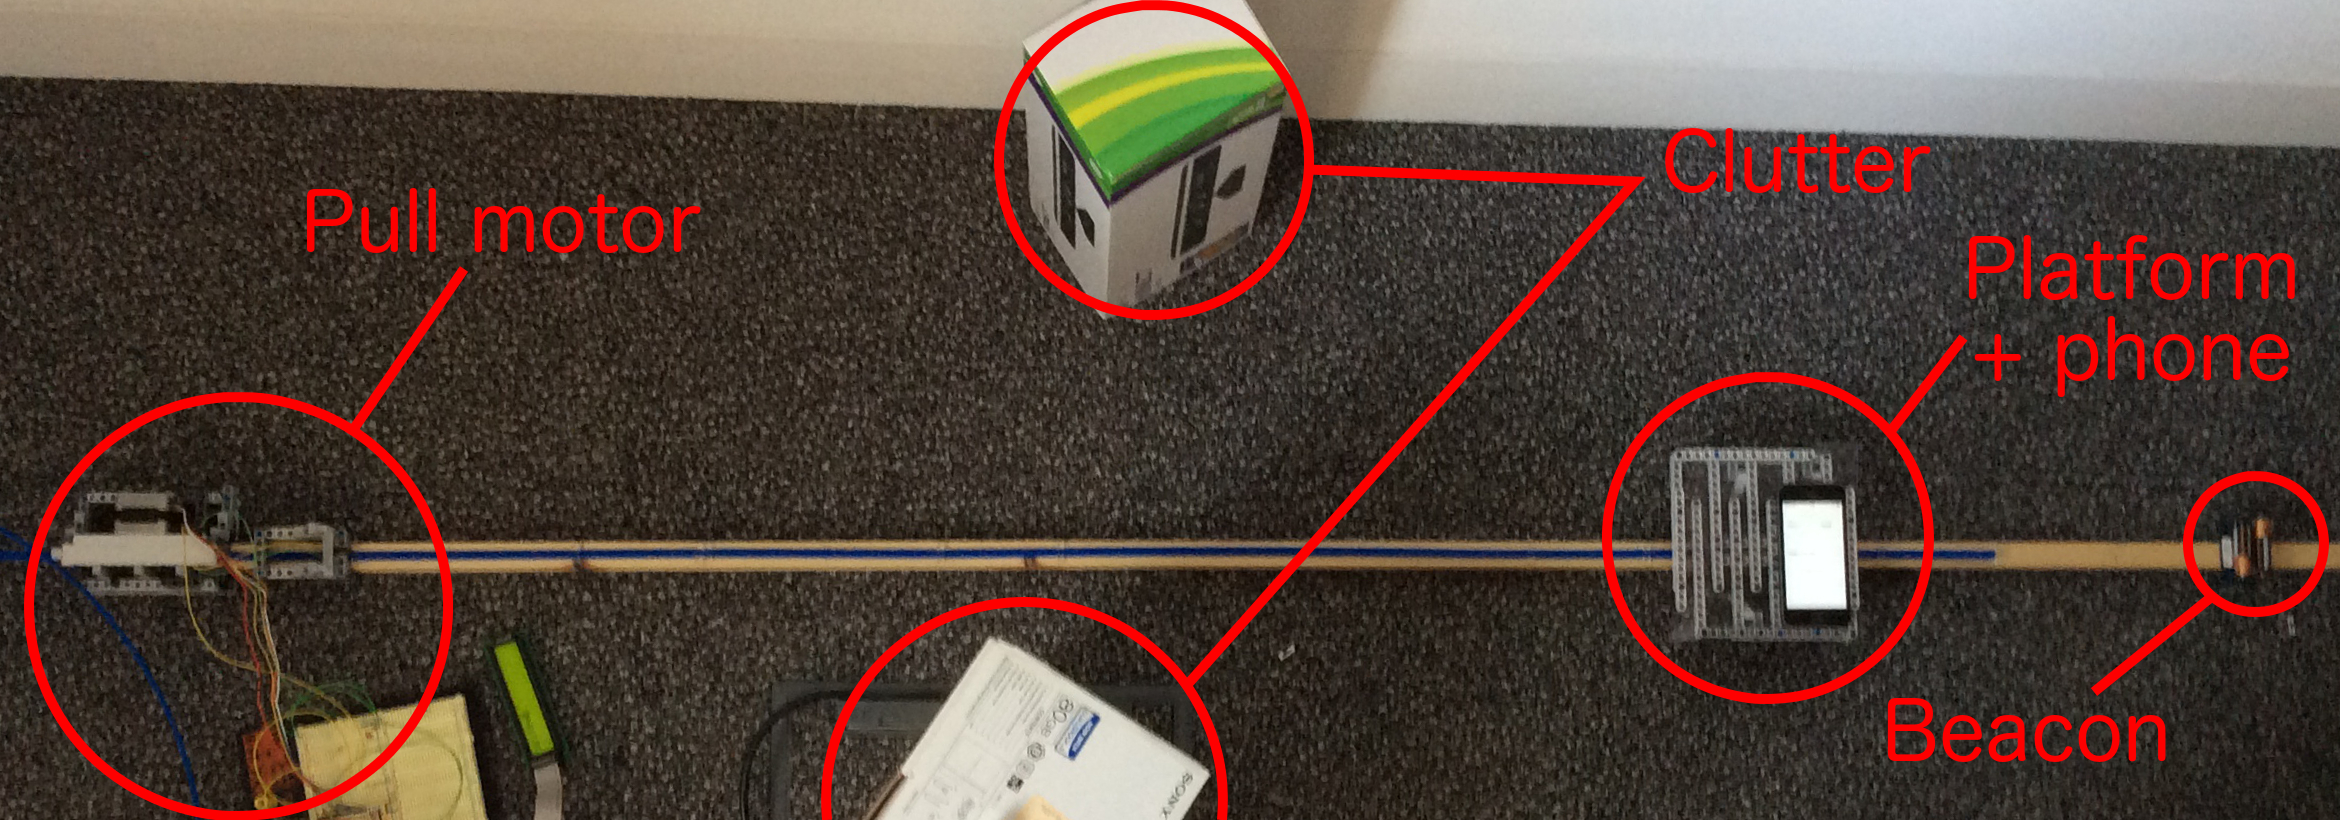
\includegraphics[width=0.8\textwidth]{images/mpi}}
    \end{subfigure}
    \caption{To measure the effect to \mpi, I built a device that pulls a platform with the \device slowly and precisely along a 3 meter path away from a beacon in a cluttered environment. Schematic and photo. The device in the photo is actually shorter than 3 meter, for clarity.}
    \label{fig:rss-pullschematic}
}

\begin{figure}[p]
    \gnuplot{rss}{mpi-combine-channels}{Received signal strength at different distances to a transmitter.}
\end{figure}

\begin{figure}[p]
    \gnuplot{rss}{mpi-split-channels}{Received signal strength at different distances to a transmitter, split out per channel.}
\end{figure}


One of the ways how \mpp can have an influence on RSS, is through \mpi.
\Mpi occurs when a signal propagates via two paths, to be received in the same point.
Depending on the length difference of the two paths, the two signals may strengthen or weaken one another (theoretically making it possible for them to cancel one another out completely).

To explore this effect I built a device that pulls a receiver (an iPhone 5) along a 3 meter track away from a BLE beacon at precisely 1mm/s (\figureref{rss}{pullschematic}).
For each package received, I log the time and the RSS.
Knowing the start-time and start-position, and the speed, I can plot the RSS against the position.
\Figureref{rss}{mpi-combine-channels} clearly shows drops and peaks in the signal that can be attributed to \mpi, however at most distances hugely different RSS values are measured.
Figure \ref{fig:rss-mpi-split-channels} shows the RSS split out by channel, and here we can see that within each channel, the RSS is fairly constant for one location, and each channel shows its own \mpids.

\begin{figure}[p]
    \gnuplot{rss}{mpi-compare}{Top three graphs are RSS of channel 37 during 3 different runs. Bottom graph is RSS of channel 38 during the third run.}
\end{figure}

\newcommand{\correlationtable}[2]{&\cellcolor{#1}#2}
\begin{table}[p]
    \begin{tabular}{ | c | r | c | c | c | c | c | c | c | c | c | }
        \cline{3-11}
        \multicolumn{2}{c |}{} &
        \multicolumn{3}{c |}{run 1} &
        \multicolumn{3}{c |}{run 2} &
        \multicolumn{3}{c |}{run 3} \\
        \cline{3-11}
        \multicolumn{2}{c|}{}
        \h{ch. 37} \h{ch. 38} \h{ch. 39}
        \h{ch. 37} \h{ch. 38} \h{ch. 39}
        \h{ch. 37} \h{ch. 38} \h{ch. 39} \\
        \hline
        \makeandinput{rss}{correlation-table-generated}
    \end{tabular}
    \caption{Pearson-correlation between multiple runs, on the same channel and different channels. Since many data points are involved, there is an extreme high certainty, and the p-value for all measurements is under machine epsilon.}
    \label{tbl:rss-mpi-correlation}
\end{table}

\Figureref{rss}{mpi-compare} shows the RSS for a single channel (37) over three runs (top three graphs), and compares this to channel 38 during the third run.
The same multipath drop pattern is visible in all three runs for one channel, while the other channel has a different pattern.
\Tableref{rss}{mpi-correlation} shows the Pearson correlation (using 1-second means) between different channels and between different runs.
The green cells show the same channel in different runs, and clearly have a much higher correlation than between different channels (the white cells).
This suggests that different channels have their \mpids at different locations, something that is to be expected, since the location of the \mpids is dependent on the wave length, thus on the radio frequency.

\fig{\gnuplot{rss}{mpi-feasibility}{Effect of a small lateral shift of the receiver and small changes in the environment on the RSS}}

It is tempting to try to use the \mpids to improve on positioning via RSS; if the drops can be mapped precisely, the combination of the three individual channels could provide a location with much precision.
For instance, if channel 37 has an RSS of -63dB, channel 38 has -50dB and channel 39 an RSS of -46dB, one could use the information from figure \ref{fig:rss-mpi-split-channels} to find a distance of 1.3m.
One of the challenges here is that the \mpids are very local, and to create fingerprints for a whole room, measurements have to be taken every couple of centimetres at least in all three dimensions.
To illustrate this, figure \ref{fig:rss-mpi-feasibility} shows in purple the original measurements, and in red the measurements taken with the receiver put on the other side of the platform, 4cm to the side of where it was in previous runs.
The same channel in both runs has a Pearson correlation of between 0.83 and 0.88, p-value < machine epsilon, considerably less than the correlation between different runs with the receiver in the same spot.
Even if such a map had been made however, \mpi is dependent on the environment, and even small changes in the environment (movement of objects or people), may invalidate a map.
Figure \ref{fig:rss-mpi-feasibility} shows this effect, purple is the base measurement, green the measurements after some small changes in the environment are made.
This time the correlation coefficient is between 0.48 and 0.66, the same as between different channels in one run.
These two effects mean that simply creating a map of an environment, even for an environment with just small changes, is not feasible, unless additional techniques are developed to combat the described problems.

\fig{
    \begin{subfigure}[b]{0.5\textwidth}
        \gnuplotscale{rss}{mpi-single-rss-10mm}{1cm}{0.55}
    \end{subfigure}
    \begin{subfigure}[b]{0.5\textwidth}
        \gnuplotscale{rss}{mpi-single-rss-100mm}{10cm}{0.55}
    \end{subfigure}
    \begin{subfigure}[b]{0.5\textwidth}
        \gnuplotscale{rss}{mpi-single-rss-400mm}{40cm}{0.55}
    \end{subfigure}
    \begin{subfigure}[b]{0.5\textwidth}
        \gnuplotscale{rss}{mpi-single-rss-1000mm}{100cm}{0.55}
    \end{subfigure}
    \caption{Using average, maximum and median strategies to determine RSS, using different distance intervals}
    \label{fig:rss-mpi-single-rss}
}

The fluctuating RSS value is unhelpful for most positioning methods.
Most positioning methods work by creating a fingerprint map, with RSS values expected to remain more or less the same over time on the same location, and on locations between two spots where fingerprints were collected, the collected RSS values should have a value between those measured in the two surrounding mapping points.
Ideally there is a smooth decrease in RSS with distance; the 6dB decrease per doubling of distance, discussed earlier in this chapter, is used, with different starting points, as an ideal reference line in this section.
Figure \figureref{rss}{mpi-single-rss} shows several strategies we may employ to remove RSS fluctuations.
I take the mean, median and maximum of the received data, over different distance intervals, and compare this to an ideal RSS line.
Taking this over a distance is artificial, since during positioning one does not know the distance travelled; therefore a method should be chosen that works well with any distance.
Figure \ref{fig:rss-mpi-single-rss} shows that both average and median follow one another very closely, with sometimes one and sometimes the other being closer to the ideal line, whereas the maximum fits less nicely but is still has nice smoothing properties.

\section{Orientation}
\label{sec:rss-rot}

The direction in which a user is facing while using a smartphone to position, also has an influence on the RSS.
This may be due to two reasons.
First, the phone itself: rotating the iPhone leads to the antenna being less or more aligned with the signal, and leads to certain parts of the phone blocking the radio signal.
Second, the user's body may either absorb or reflect the signal, leading to signal loss or gain.

\fig{
    \begin{subfigure}[b]{0.55\textwidth}
        \centering{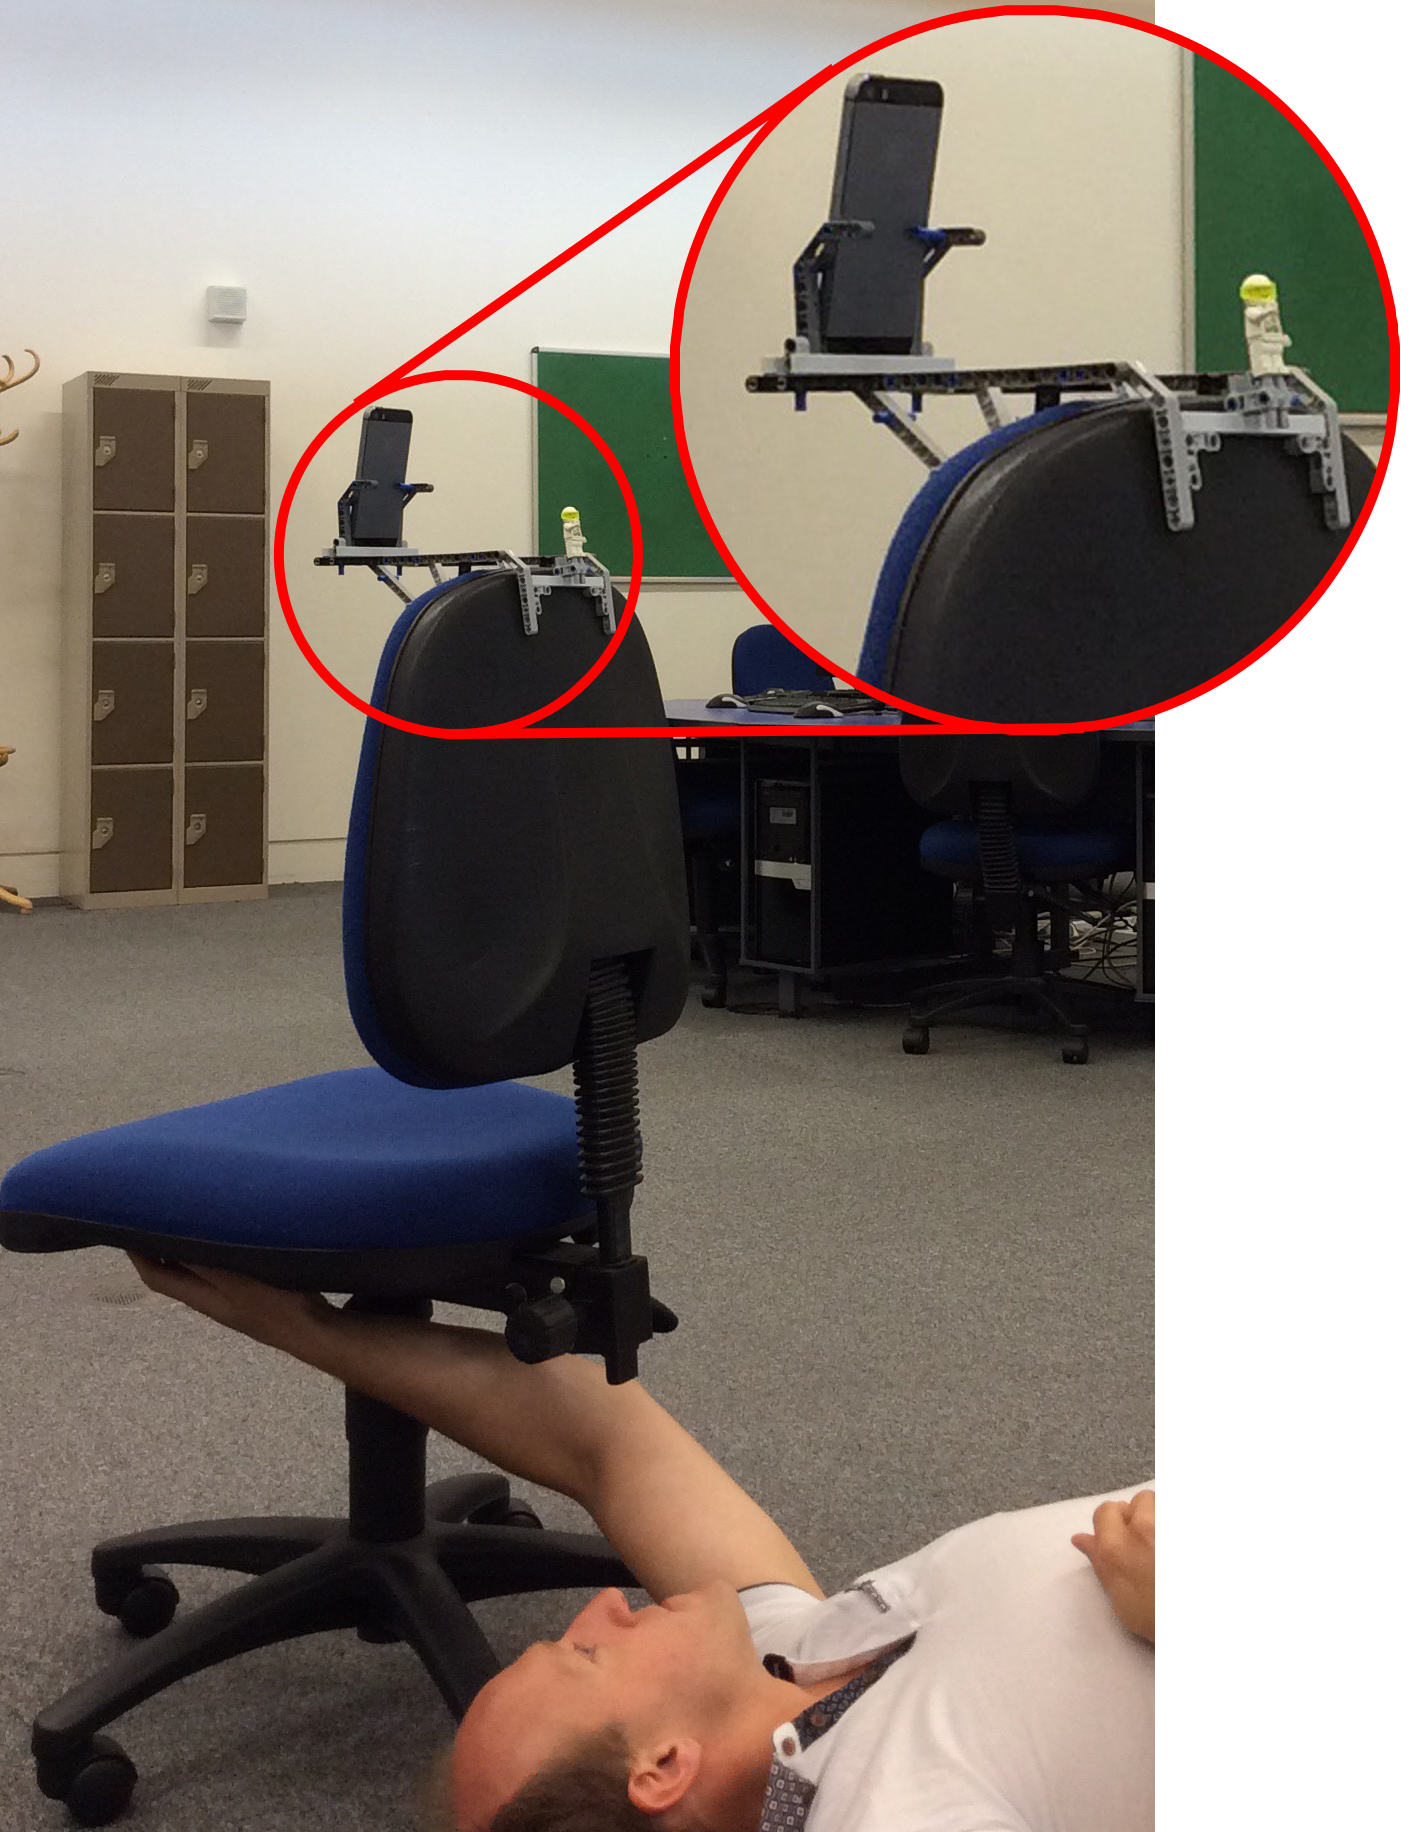
\includegraphics[width=\textwidth]{images/rot-without-body}}
        \caption{without body}
    \end{subfigure}
    \begin{subfigure}[b]{0.45\textwidth}
        \centering{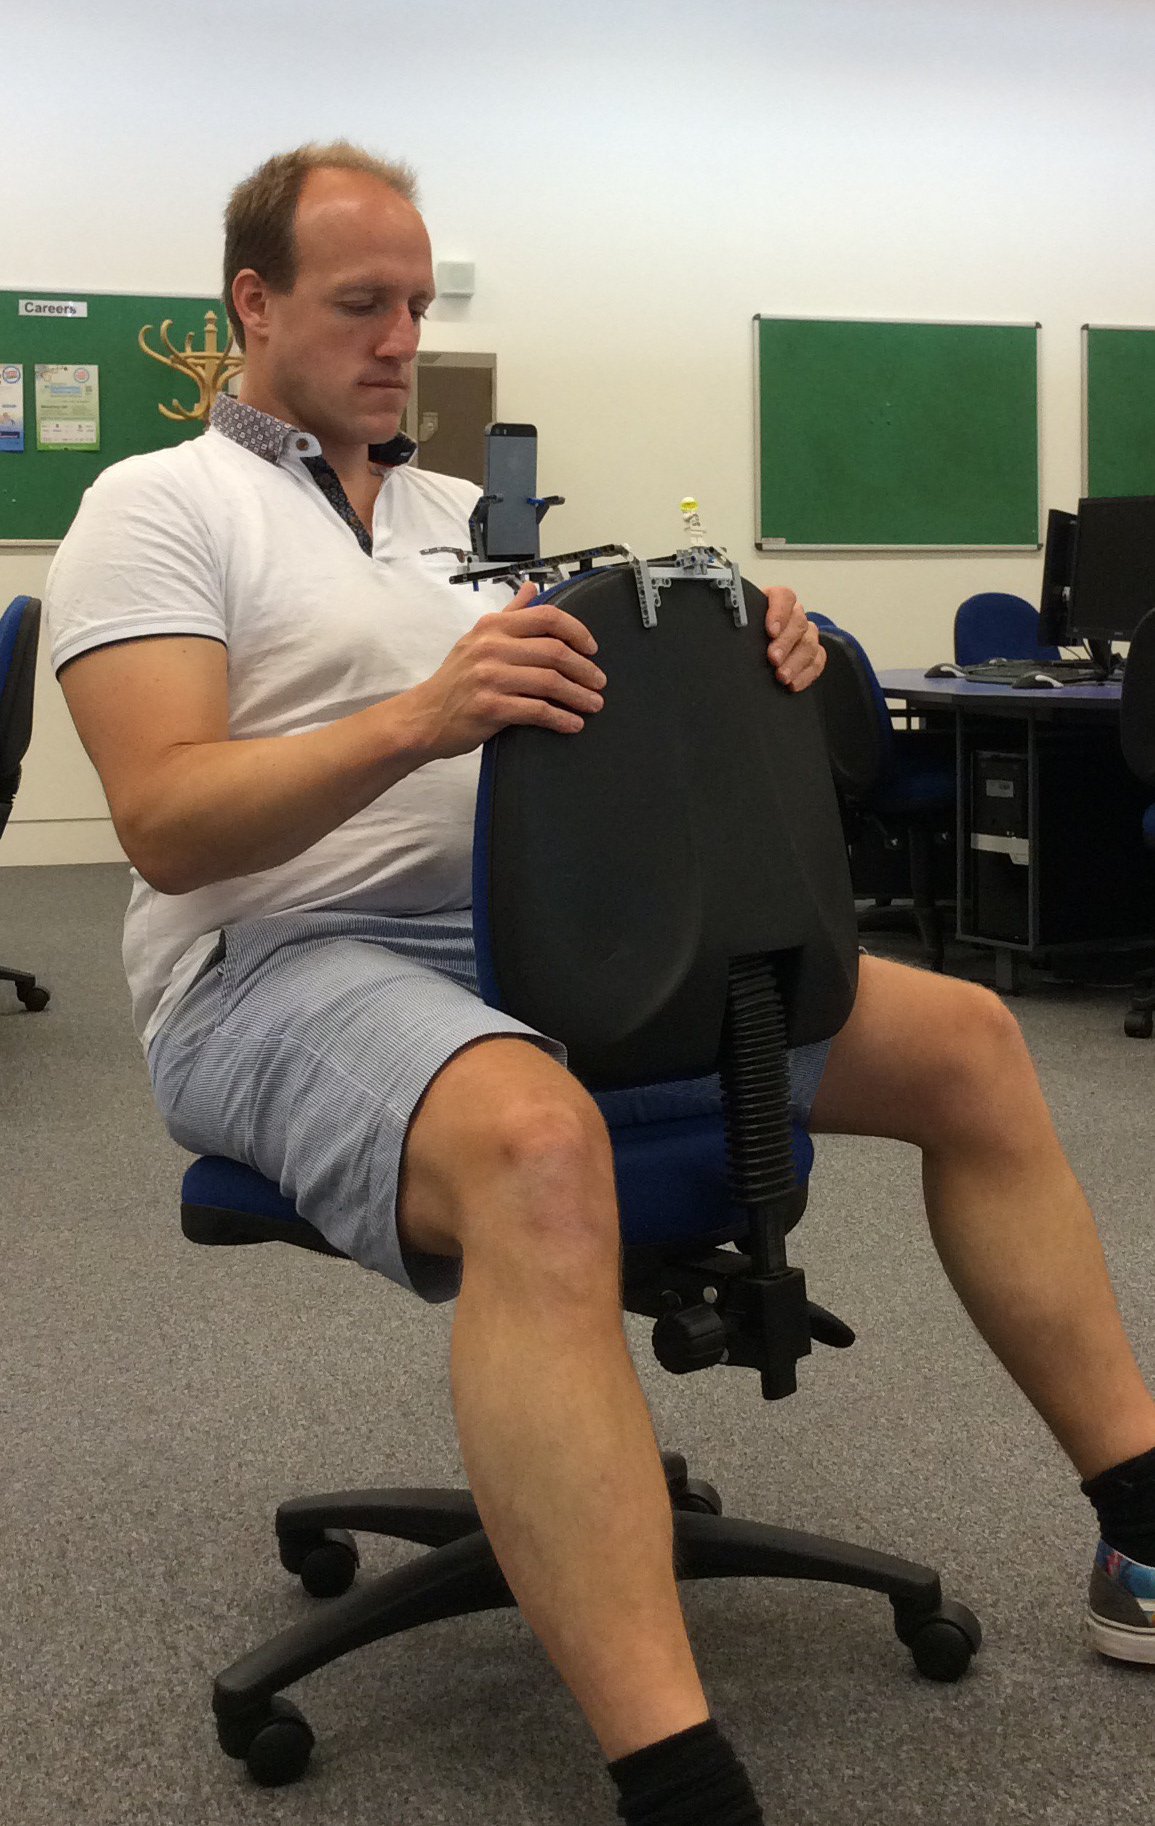
\includegraphics[width=\textwidth]{images/rot-with-body}}
        \caption{with body}
    \end{subfigure}
    \caption{Device used for measuring rotation.}
    \label{fig:rss-rot-device}
}
 

To explore these effects I built a device to rotate the \device around its axis: an small construction was added to the back of an office chair, such that a \device rotates around its axis when the chair rotates (\figureref{rss}{rot-device}).
Using the built-in compass, the heading was recorded together with the RSS.
During measurements an eye was kept on the reading from the compass and no large errors were spotted; small errors in compass accuracy do not have a major influence on the results of this section.
Two measurements were made at each location.
In 300 seconds I rotated the chair 3 $\times$ 360\tdegree, while measuring compass heading, and the RSS for a beacon placed at around 7 meters distance, while lying on the floor under the chair.
Then I sat on the chair with my body around 15 cm from the \device, and did the same 1080\tdegree rotation in 300 seconds.

\fig{
    \begin{subfigure}[b]{0.5\textwidth}
        \gnuplotscale{rss}{rot-grass}{Outside in a field}{0.55}
    \end{subfigure}
    \begin{subfigure}[b]{0.5\textwidth}
        \gnuplotscale{rss}{rot-sw02}{Indoor in a mostly open room}{0.55}
    \end{subfigure}
    \begin{subfigure}[b]{0.5\textwidth}
        \gnuplotscale{rss}{rot-corridor}{Indoor in a corridor}{0.55}
    \end{subfigure}
    \begin{subfigure}[b]{0.5\textwidth}
        \gnuplotscale{rss}{rot-sw02-nolos}{Indoor, transmitter and receiver in different rooms}{0.55}
    \end{subfigure}
    \caption{RSS under rotation, with and without a body present, in different environments.}
    \label{fig:rss-rot}
}

\Figureref{rss}{rot} shows in red the average RSS per 0.5 second, plotted against the direction the phone is facing, while I lie under the chair.
0\tdegree means that the back of phone is the facing the beacon, while at 180\tdegree the screen is facing the beacon.
Since on the iPhone 5 the \wifi/Bluetooth antenna is mounted against the back of the phone, next to the camera and flash\urlref{http://www.ifixit.com/Guide/iPhone+5+Wi-Fi+Antenna+Replacement/10897}{11 June 2014}, I expect reception to be best with that side facing the transmitter.
The blue points show the same rotation with my body on the chair, influencing the signal.
Since I'm facing the screen, at 0\tdegree the \device is between me and the beacon, while at 180\tdegree I am between the beacon and the \device.

\Figureref{rss}{rot}(a) shows that without a body present, both with the back and with the screen facing the beacon, there is optimal reception of -63dB.
Reception generally stays above -70dB, however at two points, around 120\tdegree and 240\tdegree there are large drops to around or even under -80dB, resulting in an RSS difference of 15dB in just 15\tdegree, and a 20dB difference throughout the whole rotation.
These plotted values are already averages, the extremes on different channels are even larger.

In the blue points, the effect of the body is clearly visible, shadowing the signal, resulting in a 20dB drop when between the phone and the beacon, while resulting in a slight boost of the signal when the back of the phone faces the beacon, possibly because of the reflection of the signal by the body.
Also in this case we see 20dB+ drops in the signal strength within a couple of degrees in many spots.

In \figureref{rss}{rot} the experiment is repeated in different environments, generally coming less open from (a) to (d)
In general in (b), (c) and (d) the same patterns as in (a) are visible, that at 180\tdegree the body casts a shadow on the reception, while at 0\tdegree a slight boost of signal can be seen when there is a body behind the device.
The effect is arguably smaller in the more cluttered environments, possibly because reflections result in multiple paths the signal can take around the body.
All environments show some drop orientations, where the RSS drops by 10-20dB within a couple of degrees.

\section{People moving through the room}
\label{sec:rss-busyroom}

\fig{\gnuplot{rss}{drawmeetingroom}{Schematic of meeting room in lunch setting.}}
In order to investigate how people and objects moving around a room influence RSS, 6 beacons were placed in a meeting room, together with an iPad mini as receiver on a table (\figureref{rss}{drawmeetingroom}), while a standing lunch was taking place.
All tables and chairs were moved to the side before the start of measurements.
\Figureref{rss}{busyroom} shows the RSS over time for six beacons, and how many packets were received on each channel.
Even though beacon 6 was furthest away, the highest RSS of all beacons is received from this one; this may be because it is in front of the receiver on a direct line of sight.

\begin{figure}[p]
    \begin{subfigure}[b]{0.5\textwidth}
        \gnuplotscale{rss}{busyroom-0x12}{Beacon 1}{0.55}
    \end{subfigure}
    \begin{subfigure}[b]{0.5\textwidth}
        \gnuplotscale{rss}{busyroom-0x10}{Beacon 2}{0.55}
    \end{subfigure}
    \begin{subfigure}[b]{0.5\textwidth}
        \gnuplotscale{rss}{busyroom-0x08}{Beacon 3}{0.55}
    \end{subfigure}
    \begin{subfigure}[b]{0.5\textwidth}
        \gnuplotscale{rss}{busyroom-0x06}{Beacon 4}{0.55}
    \end{subfigure}
    \begin{subfigure}[b]{0.5\textwidth}
        \gnuplotscale{rss}{busyroom-0x14}{Beacon 5}{0.55}
    \end{subfigure}
    \begin{subfigure}[b]{0.5\textwidth}
        \gnuplotscale{rss}{busyroom-0x13}{Beacon 6}{0.55}
    \end{subfigure}
    \caption{RSS and the number of packets received for the six beacons during different room occupation.}
    \label{fig:rss-busyroom}
\end{figure}

Five periods were marked using a wristwatch, these are shown in the graphs:
\begin{itemize}
    \item Period 1 (12:41-12:59): The lunch is being built up, occasionally people enter and leave the room, most of the time there are one or two people in the room.
        The door to the room is open.
    \item Period 2 (12:59-13:27): The room fills up with people, people move around, in the first half of the period there are between 15 and 20 people in the room, after which the room slowly empties.
        At the end of the period the last group of 3 people leave, and they close the door.
    \item Period 3 (13:27-13:44): The room is empty.
    \item Period 4 (13:44-13:47): Without moving any beacons or receivers, the furniture in the meeting room is put back to meeting room position, the door is closed again afterwards.
    \item Period 5 (13:47-13:52): The room is empty.
\end{itemize}

The two periods with an empty room, 3 and 5, are characterised in the graphs in \figureref{rss}{busyroom} by relatively low variance in RSS per channel, whereas period 2, when a lot of people are moving around, shows high variance, with periods 1 and 4 being somewhere in between.
The differences between period 3 and 5 likely show the influence of the furniture on the RSS, where major differences between period 1 and 3 are most likely caused by the door being open or closed.
This latter effect is especially clear with beacons 1 and 3, which are respectively in the ceiling and on the floor behind the door.
Another interesting effect is that only in beacon 6 all channels become lower during period 2.
Possibly this is because for beacon 6 the line-of-sight got interrupted during period 2, while most other beacons did not have a line-of-sight, and sometimes benefit from the extra reflection possibilities of a room full of people.

The beacons broadcast at 9.5Hz, however only once more than 6 advertising packets per second are received on average during a minute.
In the next section I look into packet loss in more detail, but it is interesting to note the large differences in packet loss between channels, and between periods.
It shows that when the RSS drops below -80dB, fewer (or sometimes hardly any) packets are received.

\section{Packet loss}
\label{sec:rss-packet-loss}
According to the \BTspec, an advertising packet should be sent on all three advertising channels within a short time.
This means that a beacon advertising at 10Hz (the beaconing rate) sends 10 packets per second on each of the three channels, heaving a 100ms \define{beaconing interval}.

A \device typically listens on one channel at a time for BLE packet, switching between the three channels.
We can therefore assume that, even though a 10Hz beacon sends 3 (channels) $\times$ 10 packets per second, a \device will at most receive 10 of these per second; any fewer would be considered packet loss.
There are many reasons why a \device may receive fewer than 10 packets, for instance:
the signal strength is too low to be received, other transmitters interfered with the signal, the \device was temporarily not ready to receive packets, or the OS discarded a packet.

As mentioned in \sectionref{rss}{smartphone}, an iOS device misses more packets if \BLE listening is active for a longer time.
To counter this, I restart BLE listening every 10 seconds in all experiments; I do not see increased packet loss at the time of restarting.

If packets are not received consistently, this may impact the positioning ability.
There is no way for the device to know whether a beacon was not observed because it is out of range, or because the packets sent by the beacon were lost.
To counter this, a \device has to scan for a number of beacon intervals; especially if beacons advertise at a low rate to save energy, this may be a problem.

To investigate packet loss I used a single beacon transmitting at 1Hz.
The measurements were done outside in a field, with no other known transmitters nearby, distance between beacon and \device 15 centimetres.
In 136 beacon intervals, 104 packets were received, a 23.5\% packet loss.

\fig{\gnuplot{rss}{packet-loss}{Packet loss for different numbers of beacons.}}
For positioning it is important to know how long one has to listen to be reasonably sure that, if a beacon has not been observed, it can not be observed in that location.
I repeated the experiment with first a single beacon set to transmit at 10Hz\footnote{The actual beacon rate of these beacons is 9.5Hz. In the text I will continue to call them 10Hz beacons, because 10Hz and 100ms intervals are easier to reason with, and because 10Hz is the setting the beacons were set to. All packet loss calculations in this section have been done with the actual rate of 9.5Hz.}, then multiple beacons, all set to 10Hz, all within a 20cm radius of the \device.
Each test was ran for one minute; the results can be seen in \figureref{rss}{packet-loss}.
It shows a packet loss of between 27 and 38\%, with a generally a higher packet loss for a larger number of beacons.
This can be explained because packets from multiple beacons may collide when sent at the same moment.

\begin{table}
    \begin{tabular}{r | c | c | c | c | c | c | c | c | c | c |}
        & \multicolumn{10}{c |}{listening time in transmission intervals} \\
        \makeandinput{rss}{packet-loss-empirical-generated}
    \end{tabular}
    \caption{Measured chance that not all beacons have been observed at different listening intervals.}
    \label{tbl:rss-packet-loss-empirical}
\end{table}

\Tableref{rss}{packet-loss-empirical} shows the results from the same experiment, but considers how often multiple subsequent packets from the same beacon were lost.
It shows that with one beacon, in 0.55\% of the cases I had still not received it after three beacon intervals.
With twenty beacons, after 10 beacon intervals, in 1.2\% of the cases I had not observed each beacon as least once.

The tests above were done in an area with minimal additional radio interference.
Looking at a more noisy environment, such as the one of \sectionref{rss}{busyroom}, there is 59\% packet loss, and even after 5.25 seconds, 50 beacon-interval at 9.5Hz, in 1\% of cases not all beacons have been observed.
This can probably be attributed to interference from \wifi and other Bluetooth devices, as well as there not always being a line-of-sight between beacon and \device.

\chapter{BLE positioning in practice}
\label{chap:architecture}

\section{RSS based positioning}
\label{sec:architecture-rss-based-positioning}
\citet{bahl2000radar} laid the foundation for positioning using \wifi signals.
The basis is a fingerprint database, containing fingerprints (the RSS, or RSS distribution, for each access point) for a large number of locations.
This database can either be filled empirically, surveying the RSS at each location; or calculated, where the RSS at each location is estimated using the positions of the access points and a radio propagation model for the environment.
They show that empirically filling the database leads to better results, however it may take much longer since a manual survey of each location is needed.

To do positioning, a measurement of the RSS of each access point at an unknown location is made, and each fingerprint in the database is compared to this measurement in order to find one or multiple close matches.
The method mostly used to find a match is (a variant of) k-nearest-neighbour.
The method works in three steps.

Firstly the set of measured RSSs, both those collected during the surveying and the positioning phase, are transformed into values needed for step two.
\citet{bahl2000radar} describes that the mean, standard deviation and median of multiple measurements at a single location was calculated, but only use the mean in the rest of the paper.

Secondly the values from the fingerprints are compared to the values found while positioning, and a distance between the two sets is determined, by a distance-function $L$.
The usual choice for the distance-function (and hence the name) is to calculate the distance in signal-space, where each signal-source is a dimension.
\citet{li2005method} described a generalised distance function (\equationref{architecture}{distance}).
\begin{equation}
    L_q = \left(\sum_{i=1}^{n}|p_i-s_i|^q\right)^{\frac{1}{q}}
    \label{eq:architecture-distance}
\end{equation}
Here $n$ is the number of signal-sources, $p_i$ the measured RSS for a source during positioning, and $s_i$ the surveyed RSS at the point to which the distance is to be calculated; different $q$ lead to different distance functions with $L_1$ being the Manhattan distance, and $L_2$ the Euclidean distance.
There seems to be no clear consensus on which $q$ gives the best result, with \citet{shin2012enhanced} using $L_1$, \citet{bahl2000radar} using $L_2$, only saying that alternatives (possibly also of another form) were briefly experimented with, and \citet{li2005method} using $L_1$, while noting that the difference with other $q$ values is not significant.
Most methods use the $L_q$ function with the $s_i$/$p_i$ in dB, \citet{li2005method} explores whether these values should alternatively use the power $P$, $1/P$, $1/P^2$ or $1/P^4$, concluding that dB works the best, but $1/P^2$ and $1/P^4$ also give good results.
Another interesting candidate is the Mahalanobis distance, use of which is explored and found to be superior by \citep{kaemarungsi2005efficient}.

Finally the calculated distances are being used to map to a position.
\citet{bahl2000radar} uses both a 1-nearest-neighbour and a k-nearest-neighbour approach, showing that the second works better (although only slightly due to some choices they made in the rest of the algorithm).
\citet{li2005method} uses a weighted-k-nearest-neighbour approach, where the nearest neighbours are being weighted by the result of the distance-calculation, and \citet{shin2012enhanced} introduced using a dynamic value for the number of neighbours $k$ to further improve the result.

\citet{pandya2003indoor} compares nearest-neighbour to other positioning methods based on RSS, and finds nearest-neighbour to work well in most cases (among which Bluetooth Classic).
Unsurprisingly, other methods from the domain of machine learning have been examined as well to do positioning, such as Gaussian Process Latent Variable Models \citep[ferris2007wifi] or Neural Networks \citep[battiti2002location].

Of these methods, the one used by \citet{bahl2000radar} is used in this report to compare against; both because the method is simple to understand and implement while giving good results, and because many other authors used this method as a base to compare against.

\section{Experiment}
\label{sec:architecture-experiment}
\fig{\gnuplot{architecture}{room}{Test bed: room SW02 in the Computer Laboratory of the University of Cambridge.}}
Room SW02 in the Computer Laboratory of the University of Cambridge is the test bed for this experiment.
The room consists of a square 12 by 12 meter main area, with several coves.
The room contains four decagonal-shaped tables with computers on them and chairs around them, as well as some other furniture.
Twenty BLE beacons were used, ten on the walls of the room, eight on the tables, one in the middle and one placed a couple of meters outside the room (\figureref{architecture}{room}).
The beacon positions were chosen such that all areas would receive BLE signals, but no specific action was taken to find optimal positions.
Each beacon broadcasts a single advertising packet, a unique \bid, on all three channels, with a rate of 10Hz; the transmitting power of all beacons is the same, and stays the same over the experiment's lifetime.
All measurements were done on a 60 by 60 cm grid, since this is the size of the floor tiles and this allowed for easy reference.

\fig{
    \centering{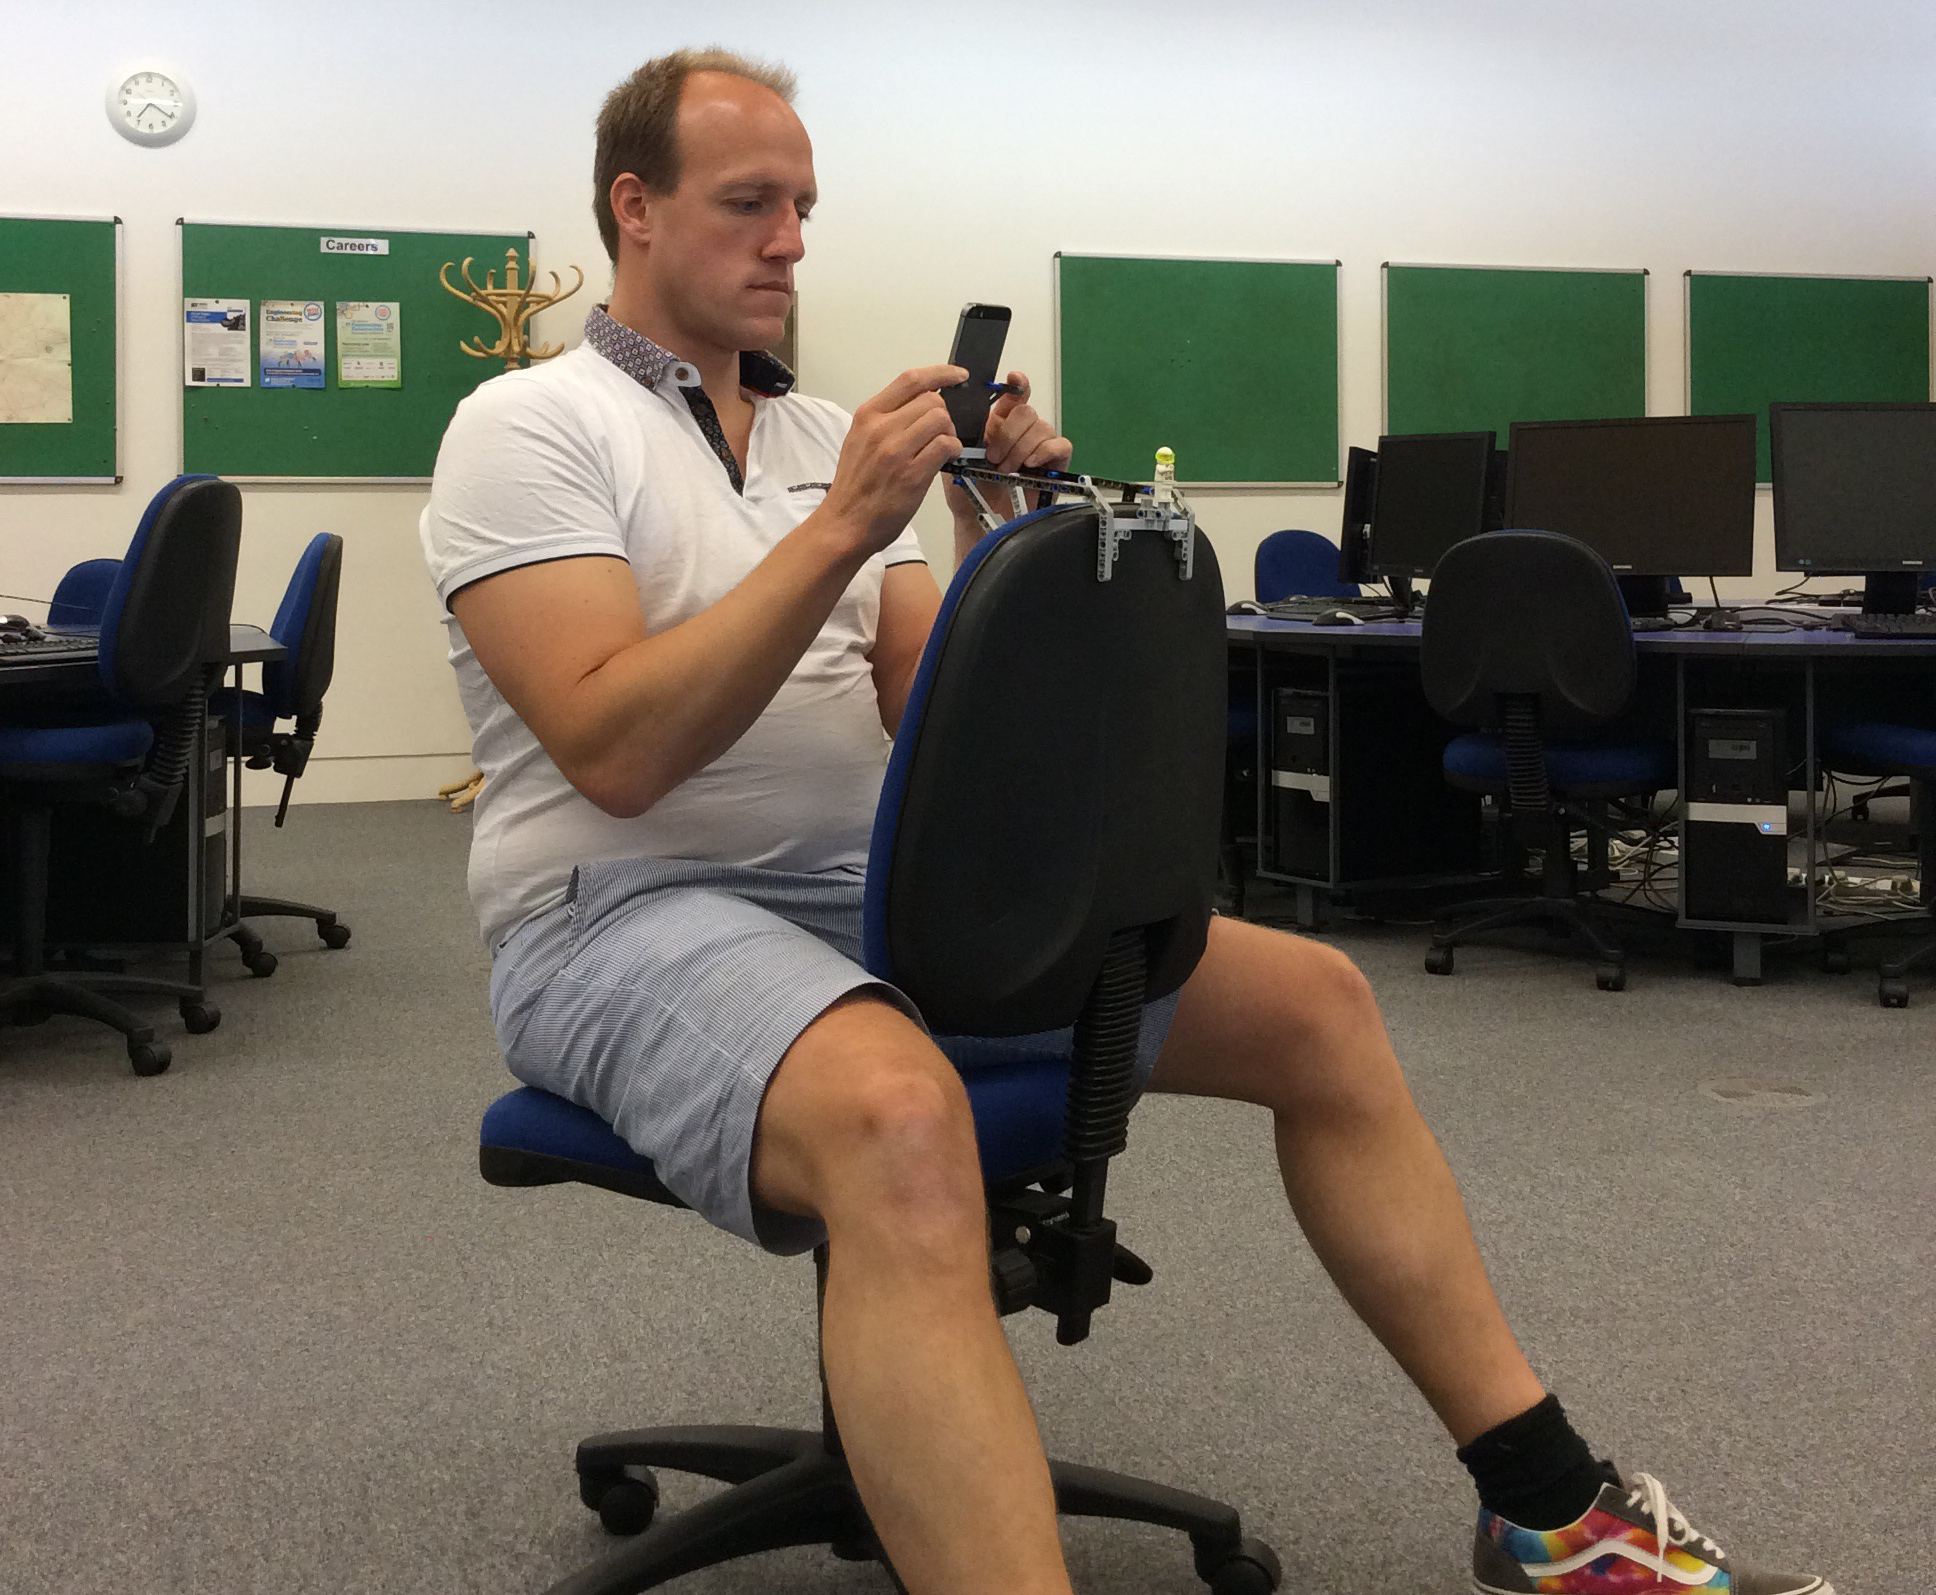
\includegraphics[width=0.7\textwidth]{images/survey}}
    \caption{Device used for surveying.}
    \label{fig:architecture-survey-device}
}

During the surveying phase, each accessible point on the grid is surveyed, by slowly moving the \device along a circle with a radius of 15 cm centred on the grid point, the back of the phone facing outwards, with a human body on the opposite side of the circle, facing the screen; the normal position for a user using the \device.
To accomplish this consistently, I adjusted the office-chair set-up of \sectionref{rss}{rot}, such that the \device now rotates along a circle instead of its axis (\figureref{architecture}{survey-device}).
For each advertisement packet received, the \bid, advertising channel, RSS and the current heading as reported by the \device's compass, is saved.
Complete 360\tdegree survey took between 3.5 and 15 seconds for each of the 226 accessible points, with a mean of 9 seconds per point.
On average 903 advertising packets were captured per point, meaning there was around 45\% packet loss.

During the positioning phase, I went to each grid point, standing naturally while holding the \device still over the grid point for two seconds, again logging the \bid, advertising channel, RSS and current heading for each received packet.
In total 670 positionings measurements were taken this way for the 226 locations, visiting each location at least twice\footnote{The intention was to visit every location three times; due to an oversight some locations were visited only twice.}.

During surveying each beacon was observed at least once at each location.
During positioning, this was not the case; this may have been because the \device was not moving, not rotating, and the listening interval was shorter.

It should be noted that both in the surveying and the positioning phase, for about 2\% of all packets no RSS information was reported by the OS; these packets were discarded.

In addition the $x$, $y$ and $z$ coordinates for each beacon were determined, and the maximum RSS on 1 meter distance.

The data gathered from this experiment allows me to compare six different positioning algorithms, and simulate how they perform under different circumstances.

\section{Positioning methods}

All positioning in this report is being done through the weighted k-nearest-neighbour algorithm.
Provided a set of distances for a single measurement to each surveyed point, ordered by distance, the average of the points belonging to the first $k$ distances is calculated, weighted by $\frac{1}{distance+\epsilon}$, to avoid division by 0; an $\epsilon$ of 0.01 was empirically found to work well.
The difference between the compared algorithms, is in how the distances are calculated, the first two steps of the nearest-neighbour algorithm as described in \sectionref{architecture}{rss-based-positioning}.
All experiments are run with $k = 5$; I found that value to be optimal in many cases, and near to optimal (within the noise range) in the other cases.

In the positioning algorithms below, the first step is always (except for ``random'') taking either the mean or the maximum RSS measured at a location.
To deal with cases when a particular beacon was not observed, that beacon is treated as having been received with an RSS of -105dB; this is 2dB lower than the lowest RSS reported for an actual packet during the experiment, and seems reasonable, since if there had been a packet with signal strength -105dB, the \device would not have noticed it.
It is possible however that another choice on how to deal with unobserved beacons gives better results; I leave this for future research.

\subsection{Random}
As a reference, the random method returns random distances for each fingerprint, after which the k-nearest-neighbours method is used to calculate a position.

\subsection{Signal Space Distance (SSD)}
The method described in \citet{bahl2000radar}, using dB for the RSS, and the $L_2$ distance function (\equationref{architecture}{distance}).
As in \citet{bahl2000radar}, the mean RSS over all received packets is used both in the surveying and the positioning data.
Only one fingerprint per position is taken, unlike \citet{bahl2000radar}, who created four fingerprints in four different directions.

\subsection{Signal Space Distance with Orientation (SSD-O)}
\label{sec:architecture-ssd-o}
In \sectionref{rss}{rot} I showed that the direction of measurement has a huge influence on the RSS.
\citet{bahl2000radar} recognised this in \wifi, and surveyed in four directions; during positioning however they had no way to determine the orientation, and all four directions were considered equally during positioning.
\citet{king2006compass} considered how knowledge of the orientation improves positioning.
They surveyed in eight directions, and considered different ways of combining these into ad-hoc fingerprints during positioning.

I consider a variant of King's method, using the Signal Space Distance, but taking orientation into consideration: SSD-O.
Unlike the \wifi surveying used by \citet{bahl2000radar} and \citet{king2006compass}, I survey continuously while turning 360\tdegree.
For each packet received, the heading as reported by the \device's compass is stored in the database, with the \bid and the RSS.
While positioning, the \device is expected to not be rotating much; the average heading $h_p$ of the device is used to build an ad-hoc fingerprinting database.
This database is built using the mean RSS, where at each location, for each beacon, only those packets are considered that were received during surveying with a heading $h_s$ where $h_p - \alpha < h_s < h_p + \alpha$.
A value of 60\tdegree for $\alpha$ was found to work best (see \sectionref{architecture}{measurements}).
In order to not have to calculate the ad-hoc fingerprint database for each positioning, the experiment was run with 360 pre-calculated fingerprint databases, one per 1\tdegree, where for each positioning the closest database is used.
For example, if the average heading during positioning is 34.6\tdegree, the pre-calculated database at 35\tdegree will be used, which is built using all surveying packets that were received between 335\tdegree and 95\tdegree.

It should be noted that this method is dependent on the accuracy of the built-in compass.
During surveying and positioning I kept an eye on the compass reading, and noticed nothing absurd, however no further effort was made to check how accurate the compass is.
During a similar experiment in another part of the building, I did notice huge compass fluctuations.
In \sectionref{architecture}{measurements-ssd-o}, I explore the influence that a potential compass-error has on this method.

\subsection{\BRP (\aBRP)}
\label{sec:architecture-brp}
\begin{figure}[p]
    \begin{subfigure}[b]{0.5\textwidth}
        \gnuplotscale{architecture}{rss-cloud-2.0s}{2.0s}{0.55}
    \end{subfigure}
    \begin{subfigure}[b]{0.5\textwidth}
        \gnuplotscale{architecture}{rss-cloud-1.0s}{1.0s}{0.55}
    \end{subfigure}
    \begin{subfigure}[b]{0.5\textwidth}
        \gnuplotscale{architecture}{rss-cloud-0.5s}{0.5s}{0.55}
    \end{subfigure}
    \begin{subfigure}[b]{0.5\textwidth}
        \gnuplotscale{architecture}{rss-cloud-0.2s}{0.2s}{0.55}
    \end{subfigure}
    \caption{Relation between the maximum RSS per beacon measured in a spot during surveying and positioning, for different listening times. If a beacon is not observed, it is assigned an RSS of -105dB.}
    \label{fig:architecture-rss-cloud}
\end{figure}

I introduce \BRP to do positioning with \BLE, taking into account some of the radio propagation properties of BLE that were described in \chapterref{rss}. 
Most notably, the method recognises that some beacons may be temporarily blacked-out; they may be received at much lower RSS or not at all due to \mpi, orientation, body shadowing or packet loss.

\aBRP uses the same k-nearest-neighbour approach as the previous methods, however since it does not calculate distance between a fingerprint and the measurement in a multi-dimensional signal space, it intuitively makes more sense to talk about a \define{penalty function} in this context.
The function gives penalty points for each way in which a fingerprint does not agree with a positioning measurement.
This syntactic difference does not change its semantics however: penalties are calculated for each fingerprint in the database, and the ones with the lowest penalties are selected to be averaged.

\BRP recognises that, once during surveying the maximum RSS $s_i$ in an area has been determined for a certain beacon, it is unlikely that during positioning a much higher RSS $p_i$ will be measured at that point\footnote{I experimented whether taking the 95th or 99th percentile would give me better results than the maximum, however there was no obvious advantage.}.
This means that $p_i \gg s_i$ should result in a large penalty.
On the other hand, having measured a much lower RSS may be the result of \mpi, antenna orientation, body shadowing, or packet loss, and is not a strong indicator that a particular position should be discarded; hence $p_i \ll s_i$ should not carry a large penalty.
Obviously the lowest penalty is given if $p_i \approx s_i$.
By adding the individual penalties given per beacon together, the full penalty for a fingerprint is obtained.

\Figureref{architecture}{rss-cloud} shows how $s_i$ relates to the $p_i$ on the same location.
The figures show that $p_i$ is on average a couple of dB lower than $s_i$; it shows that my assumption that $p_i$ is not much higher than $s_i$ is correct, and shows that there are many situations where $p_i \ll s_i$.
Shorter listening intervals lead to a higher difference between $s_i$ and $p_i$, which is to be expected since $p_i$ is the maximum for all packets, and a shorter listening period will give a smaller maximum on average.
The points on the left side, where $p_i$ = -105dB indicate those situations when a certain beacon was not observed during the listening interval.

\fig{\gnuplot{architecture}{penalty}{Penalty function for \aBRP, as compared to SSD}}

The following penalty function was empirically found to work well.
It is based on $d_i$, which is the difference between $p_i$ and $s_i$.
A positive $d_i$ indicates that the measured RSS during positioning is larger than the RSS surveyed for a candidate location.
\begin{equation}
    L = \begin{cases}
        |d_i| \times 100000 +3.042  & \text{if } d_i > 3dB \\
        |d_i| +0.042                & \text{if } 0dB < d_i \leq 3dB \\
        |d_i+4.2| \times 0.01       & \text{if } -10dB < d_i \leq 0dB \\
        |d_i| \times 0.125          & \text{if } d_i \leq -10dB 
    \end{cases}
    \label{eq:architecture-BRP-punishment}
\end{equation}
This penalty function is shown in \figureref{architecture}{penalty} and compared to the (scaled) Euclidean distance function.

The function can be understood by realising that for $d_i > 0dB$, large and very large penalties are given (top two lines).
For $d_i < -10$dB, penalties start with a large offset, but increase only slowly as $d_i$ decreases.
The part in between has very low penalties with a minimum of 0 at $d_i = -4.2$.
This is the average $d_i$ for the 2 second listening interval.

Many of the penalty offsets, factors and cut-offs in the \aBRP penalty function have been discovered by manual tweaking.
The function has been optimised for performance on the 2 second listening interval, however while keeping performance in other situations in mind as well.
Considering the changes in $d_i$ distribution for different listening intervals, as shown in \figureref{architecture}{rss-cloud}, optimising for other listening intervals will probably lead to other parameters.
Further research will have to show whether a version that dynamically adapts to the listening interval, or explicitly takes unobserved beacons into account, is feasible.

\subsection{\BRP with Orientation (\aBRP-O)}
Taking orientation into account in \aBRP, in the same way that SSD-O does for SSD, is an obvious extension.
It should be noted however that \aBRP is specifically designed to have a certain resistance to signal drops, including those from orientation.
The expectation therefore is that \aBRP-O will bring less benefit to \aBRP than SSD-O brings to SSD.

In SSD-O, $\alpha$ = 60\tdegree was found to work best; in \aBRP-O $\alpha$ = 90\tdegree works best.

\subsection{\BRP with Radio Propagation Model (\aBRP-RPM)}
Whereas \aBRP uses a surveyed database of fingerprints, \aBRP-RPM estimates the maximum RSS on a specific location using a radio propagation model.
\citet{bahl2000radar} describe a radio propagation model used for \wifi signals, which uses the layout of the building, and a Wall Attenuation Factor to estimate RSS at different locations.
Such a model does not work well for \aBRP however, since \aBRP expects the fingerprints to be the maximum receivable RSS in that area, and the model in \citet{bahl2000radar} tries to have a low average error.
Instead I use a simplified model for maximum expected RSS at a position.

Knowing that RSS is in decibel of the power, and the power decreases quadratically with distance, one can calculate the RSS $R(x)$ for a radio signal in empty space at distance x from the transmitter, if the RSS at 1 meter distance $R_0$ is known.
\begin{equation}
    R(x) = R_0 - 10 \times \, ^{10}\log(x^2) = R_0 - 20 \times \, ^{10}\log(x)
\end{equation}

By measuring the RSS at one meter for each beacon (if all beacons are similar, this only has to be measured for one beacon), this formula can be used to estimate the maximum RSS at any location.
Using this formula, the $R_0$ and the $x$, $y$ and $z$ coordinates of all beacons, an estimated RSS can be calculated at each location.
It should be noted that \mpp and other radio propagation properties can result in the actual RSS in a spot being higher than the one estimated this way, however it is hoped that this is seldom more than 3 dB, and \equationref{architecture}{BRP-punishment} already allows for this, only adding severe penalties for more than 3 dB difference.

\section{Measurements}
\label{sec:architecture-measurements}
\begin{figure}[p]
    \begin{subfigure}[b]{0.5\textwidth}
        \gnuplotscale{architecture}{heatmap-f-mean}{mean (SSD)}{0.55}
    \end{subfigure}
    \begin{subfigure}[b]{0.5\textwidth}
        \gnuplotscale{architecture}{heatmap-f-ssd-o-0}{mean, direction north (SSD-O)}{0.55}
    \end{subfigure}
    \begin{subfigure}[b]{0.5\textwidth}
        \gnuplotscale{architecture}{heatmap-f-max}{maximum (\aBRP)}{0.55}
    \end{subfigure}
    \begin{subfigure}[b]{0.5\textwidth}
        \gnuplotscale{architecture}{heatmap-f-brp-o-0}{maximum, direction north (\aBRP-O)}{0.55}
    \end{subfigure}
    \begin{subfigure}[b]{0.5\textwidth}
        \gnuplotscale{architecture}{heatmap-f-rpm}{estimated (\aBRP-RPM)}{0.55}
    \end{subfigure}
    \begin{subfigure}[b]{0.5\textwidth}
        \gnuplotscale{architecture}{heatmap-13-max}{maximum (\aBRP), other beacon}{0.55}
    \end{subfigure}
    \caption{Each method uses its own fingerprint database; shown the RSS of the central beacon in each database}
    \label{fig:architecture-heatmaps}
\end{figure}

\Figureref{architecture}{heatmaps} shows the RSS for a single beacon in the different fingerprint databases.
The RSS looks as expected; RSS generally decreases with distance to the beacon.
The SSD-O fingerprint has slightly higher averages than the SSD south of the beacon, and slightly lower north of the beacon, because of body shadowing.
The maximum RSS (as shown in (c)) is about 10dB higher than the mean (this is generally consistent with the results from \figureref{rss}{mpi-combine-channels}).

\fig{\gnuplot{architecture}{results}{Errors for the six positioning methods and two combined methods}}

\subsection{Random}
Using a (deterministic) random distance function gives a mean error of around 6 meters, something that was expected considering that the k-nearest-neighbour algorithm will have a tendency to choose positions in the middle of the room as it averages $k$ positions.
Obviously this would grow with the size of the test bed; it does give a lower bound for positioning.
\subsection{Signal Space Distance}
\fig{\gnuplot{architecture}{positioning-errors-SSD}{Positioning errors using SSD, colour indicates average error, arrows indicate the direction where the algorithm calculated the \device to be.}}
SSD gives a median error of 1.08 meter, and counts as the positioning function the other ones are evaluated against.
\Figureref{architecture}{positioning-errors-SSD} shows that some areas in the room have a larger mean error than other areas, while the arrows show no obvious direction in which the errors lie.

In general positioning seems to be more accurate close to the walls; one explanation may be that orientation and \mpi influence the reception less close to the wall than in the middle of the room, because reflection off the wall compensates for that.
I have been unable to find clear evidence for this however.

\subsection{Signal Space Distance with Orientation}
\label{sec:architecture-measurements-ssd-o}
\fig{\gnuplot{architecture}{ssd-o-parameter-effect}{Positioning errors using SSD-O, for different values for $\alpha$, and different number of databases.}}
\Figureref{architecture}{results} shows that using the internal compass to take orientation into account can improve positioning performance; in the experiment the error was between 10\%-20\% lower for SSD-O versus SSD, and even more for the upper percentiles.

The average heading stored for all packets received at a single positioning is calculated (since the \device is held still during positioning, all spread in heading is due to noise), and a pre-calculated fingerprint database is used which only considered all surveyed packages in an angle of $\alpha$ = 60\tdegree to the left and right of this heading.
In total, 360 SSD-O databases were pre-calculated, one per 1\tdegree.

\Figureref{architecture}{ssd-o-parameter-effect} shows how the median error changes, if $\alpha$ and the number of databases are adjusted.
It shows that an $\alpha$ of 45\tdegree or 60\tdegree performs best, however all databases between 30\tdegree and 90\tdegree perform close to one another.
Intuitively one may expect databases with smaller $\alpha$ to perform better, however each location was only surveyed for 9 seconds on average, meaning that each 30\tdegree part was only surveyed during 0.75 seconds, or 7.5 beacon intervals, on average.
\Sectionref{rss}{packet-loss} showed that in 7.5 beacon intervals, there is still a reasonable chance that a certain beacon was not observed; and even if all beacons were observed, multiple packets are preferred to come to a good mean.
Indeed 1\% of values in the SSD-O fingerprint database for $\alpha$ = 15 is -105dB.

A single fingerprint database is in the order of 20 bytes per $m^2$ (see \sectionref{architecture}{database}); if we need 360 databases (one per \tdegree), this increases to 7 kilobyte.
\Figureref{architecture}{ssd-o-parameter-effect} shows that more databases generally improve performance, however especially above 36 the change is small, and even with just 3 or 4 databases, performance is better than in the SSD case (the 180\tdegree line).
How many databases should be pre-calculated depends on the application and the amount of storage space available for the databases.

\fig{\gnuplot{architecture}{positioning-compass-error-ssd}{Influence of compass error on SSD-O.}}
SSD-O uses the device's compass to determine orientation.
During surveying and positioning no obvious errors in the orientation reported by the \device's compass were observed, however the compass accuracy was not measured.
In other environment the \device's compass was seen to give errors that were off by 90\tdegree, therefore it is interesting to look at what happens when the compass device gives wrong readings.
For \figureref{architecture}{positioning-compass-error-ssd} the heading readings during the positioning were offset by different values.
The figure shows that SSD-O outperforms SSD with errors of less than 30-60\tdegree.

\subsection{\BRP}
\Figureref{architecture}{results} shows that \aBRP slightly outperforms SSD, however not by much, and worse than SSD-O.
It is still interesting because it gives an alternative positioning method, based on the radio properties of BLE, and because it is more resilient against unobserved beacons, either because of a shorter listening period (\sectionref{architecture}{short-walk}) or because of other reasons (\sectionref{architecture}{dying-beacons}).

It is also of interest that \aBRP and SSD have errors in different locations; a combination of the two could be used to further improve positioning, although the way in which to make this combination needs further research.
As \figureref{architecture}{results} shows, taking the average of the locations returned by SSD and \aBRP (labelled SSD+\aBRP), already results in a positioning method that is better than either one.

\subsection{\BRP with Orientation}
\fig{\gnuplot{architecture}{brp-o-parameter-effect}{Positioning errors using \aBRP-O, for different values for $\alpha$, and different number of databases.}}
As expected, \aBRP-O does not give the same performance benefits over \aBRP as SSD-O has over SSD.
It has the same median performance as \aBRP, it does however have a lower mean (1.19m vs 1.25m) and 75th percentile (1.58m vs 1.67m).
It should be noted however that the \aBRP penalty function was optimised for the \aBRP situation, and different parameters are needed for the \aBRP-O function.
In \sectionref{architecture}{short-walk} I show that \aBRP-O does outperform all other methods on shorter listening intervals.

I change the same parameters for \aBRP-O as I did for SSD-O.
A larger $\alpha$ gives a smaller error; it is possible that choosing different parameters for the penalty function results in different optimal $\alpha$.
As \figureref{architecture}{brp-o-parameter-effect} shows, reduction of the number of databases to 36 or even 12 or 6 can be done without sacrificing much accuracy; some $\alpha$ lines even seem to increase with fewer databases, I expect this to be by chance though.

\Figureref{architecture}{results} shows that, although \aBRP-O performs worse than SSD-O, taking the average of the locations of both (labelled SSD-O+\aBRP-O), results in better performance, especially for those locations with a larger error.

\subsection{\BRP-Radio Propagation Model}
\label{sec:architecture-measurements-brp-rpm}
\aBRP-RPM performs twice as bad as SSD and \aBRP, however the main advantage is that no surveying has to be done, and the database is extremely small; it only needs to contain information on each beacon's location and transmit power.
Efficiently encoded this information is 12 bytes\footnote{
    Assume we want a world-wide coordinate system with a resolution in the cm-range.
    Earth's surface area is 510,072,000 $km^2$; any usable coordinate is between -10km and +200km in height, giving 107,115,120,000 $km^3$, or $10^{26} cm^3$ to address -- any errors due to the earth not being flat fall within error margins.
    11 bytes covers $3\times 10^{26}$ addresses.
    The RSS value is only 1 byte, hence 12 byte is enough.
}, so a beacon could include this information in its advertising packet, completely removing the need for a database.

\section{Change parameters}
During this section I look at the performance of the different methods when certain parameters in the system are changed.
Throughout the section the median error is used for the performance; I have found this to be a good indicator for the performance of the whole system.

In sections \ref{sec:architecture-number-beacons}, \ref{sec:architecture-dying-beacons} and \ref{sec:architecture-number-surveyed-points} I ``randomly'' remove beacons and surveying points.
In these cases the results are gotten by doing 100 iterations, removing the beacons and points in a different order each time.
The order in which the beacons and points are removed is determined by sorting md5-hashes of the \bid/point coordinates and the iteration number, resulting in a deterministic pseudo-random order.
The median error plotted is the average of the median errors of the 100 iterations.


\subsection{Number of beacons}
\label{sec:architecture-number-beacons}
\fig{\gnuplot{architecture}{beaconcount}{Effect of the number of beacons}}
Every beacon added improves positioning, but results in diminishing return.
The test bed contained 20 beacons, about 0.1 per $m^2$.
\Figureref{architecture}{beaconcount} shows all methods having gradually increasing errors when fewer beacons are used.
This effect is slightly smaller in the \aBRP-based methods, and they outperform SSD-O for a small number of beacons.


\subsection{Unobserved beacons}
\label{sec:architecture-dying-beacons}
\fig{\gnuplot{architecture}{livebeaconcount}{Effect of unobserved beacons}}
In the previous section, I considered what happens if there are fewer beacons, both during surveying and positioning.
In this section I explore what happens if the beacons were seen during surveying (hence are present in the fingerprint database), but not during positioning.
This may be because a beacon was switched off, the battery died or the beacon was purposefully removed in a denial-of-service attack.
Since \wifi access points are plugged in to mains, and they are usually in locations not easily accessible to attackers, they are less likely to suffer from the latter two failures than BLE beacons.

Another reason that a beacon may be unobserved is that all packets from the beacon during the listening interval were lost.
\Sectionref{rss}{busyroom} shows that there is a lot of packet loss, and beacons may not be observed, even after several beaconing intervals.
This specific situation is investigated more in \sectionref{architecture}{short-walk}, where the listening intervals are shortened.

If no packets have been received from a beacon during either surveying or positioning, the algorithms used set its average and maximum RSS -105dB.

\Figureref{architecture}{livebeaconcount} shows that the both SSD based methods are very sensitive to unobserved beacons.
A single unobserved beacon almost doubles the mean error for both methods.
The \aBRP methods however are designed to resist blacked-out beacons, and only show gradually increasing errors in a situation where beacons are not observed.
Even with a single unobserved beacon, \aBRP outperforms SSD-O and SSD by having a 35\% and 42\% smaller median error.

\subsection{Positioning listening length}
\label{sec:architecture-short-walk}
\fig{\gnuplot{architecture}{unobserved}{Percentage of positionings with unobserved beacons}}
\fig{\gnuplot{architecture}{short-walk}{Effect of positioning listening interval on median error}}
As described in \sectionref{architecture}{experiment}, positioning was done by listening at a single location for 2 seconds.
On average, 197 packets were received during one positioning, meaning a 48\% packet loss (based on the actual 9.5Hz advertising rate for the beacons).
\Figureref{architecture}{unobserved} shows that only 1.5\% of positionings fail to observe all beacons with a 2 second listening interval, but at shorter intervals, more positionings do not observe all beacons.

\Sectionref{architecture}{dying-beacons} shows the effect that unobserved beacons have on positioning.
In addition to beacons being unobserved, a shorter listening interval also leads to fewer packets for those beacons that are observed, meaning that the calculated mean or maximum RSS is less accurate.

\Figureref{architecture}{short-walk} shows the effects of a shorter listening period.
Decreasing the listening period from 2 seconds, the error increases slightly until about 0.7 seconds, when it sharply increases for the SSD based methods, and less, but still considerate, for \aBRP based methods.

With 30\% of positionings having at least one beacon unobserved at 0.7 seconds (\figureref{architecture}{unobserved}), and the knowledge from \sectionref{architecture}{dying-beacons}, this result is not unexpected.

The beacons used for this experiment broadcast at 9.5Hz, meaning that 0.7 seconds is a 6.3 beacon intervals.
I believe that good positioning is a lot harder at listening intervals of less than 6 beacon intervals; this is especially a problem if beacons are set to lower beaconing rates in order to save energy.

\subsection{Number of surveyed points}
\label{sec:architecture-number-surveyed-points}
\fig{\gnuplot{architecture}{surveypointpart}{Effect of reducing the number of points surveyed}}
In order to see the effect of the number of points in the fingerprint database, I removed survey points from the fingerprint database, while still using the same data for positioning.
The points were removed in the deterministically-random way described before.

As \figureref{architecture}{surveypointpart} shows, removing fingerprints reduces accuracy, as one might expect.
Reducing the database to 100 points, a 55\% decrease, only increases the median error with around 15\%, however removing more points results in a stronger increase in median error.

The \aBRP based methods are shown to be more resilient against removal of even more surveying points than the SSD based methods, even though I do not have an explanation for this.
The \aBRP-RPM does not use a fingerprint database, and therefore always performs equally good.

\section{Discussion}
\label{sec:architecture-discussion}
In this chapter I demonstrated that \ptfp using BLE is possible using a beacons and an iPhone, and I introduced some new algorithms and showed they work.
It was intended as such, and in no way does it answer all issues in BLE positioning.
In this section I discuss some factors that have not been taken into account.
Each of them lends itself to further research.

The device used to do the surveying and the positioning was the same physical device.
Do different devices return different RSS for the same signal, and if so, how can a positioning method correct for that?

The test was done in a 2D environment; applying this to a 3D environment is not trivial.
Indoor environments often span multiple floors and beacons can be received through floors and ceilings.
A 2 meter error horizontally is probably acceptable in many positioning scenarios, while 2 meter vertically may position you on a different floor.

The test bed environment was mostly deserted during both surveying and positioning.
\Sectionref{rss}{busyroom} shows that people moving around results in large RSS fluctuations in both directions.
How do the positioning methods in this report perform in an environment where many people move around.

Finally the test bed used in this report is a relatively open space.
Walls may block or weaken BLE signals.
Because \aBRP is designed to be less sensitive to such signal drops, it may ``miss'' these hints about on which side of a wall it is.
I expect \aBRP to perform as well as SSD in this, provided there are enough beacons on both side of the wall, however further research will have to show this.

\section{Access to the fingerprint database}
\label{sec:architecture-database}
One question we have not dealt with above is how the \device has access to the fingerprint database.
Although this does not influence the results of the positioning, it is interesting to consider, especially in the light of chapter \ref{chap:security} on privacy and security.
The database size depends on the area that is being mapped, around 20 bytes per $m^2$ gives a fair estimation\footnote{Assume a $10,000m^2$ area that we want to map.
    I assume a compact data format, which starts with a list of beacons, and then surveyed information, one survey point per meter, 10,000 survey points in total.
    This results in 10,000 data points, for each I'll store the RSS of the 20 \begin{em}closest\end{em} beacons.
    Since the coordinates for all beacons are known, and the coordinates for each surveyed point are known, the \device can calculate the 20 closest points.
    The RSS was returned by all test devices as signed 8-bit value; some space could be saved by recognising that the interesting values for RSS all lie within a 6-bit range, but 8 bits will give us a good idea of size.

    This means that for the beacon-list, we need 8 bytes per beacon (2 byte \bid and 2 bytes per $x$, $y$ and $z$ coordinate), and for the actual RSS $20 \times 1 byte$ per position.
    Assuming a beacon every 5 meters, 400 in total, the map will be $some overhead + 400 \times 8 + 10,000 \times 20 \times 1 = 200.4 kilobyte$, which results in about 20 bytes per $m^2$.
    It should be noted that the survey resolution of one measurement per $m^2$ may be too low or high (\figureref{architecture}{surveypointpart} suggests that a lower resolution may perform only a bit worse), or that the 20 closest beacons are too many or too little, but this gives at the least an idea for the size of the map.
}, resulting in about 50 kilobyte for the average Tesco Superstore\urlref{http://www.tescoplc.com/files/pdf/results/2014/prelim/prelim_2013-14_analyst_pack.pdf}{10 June 2014}, up to 1 megabyte for large museums such as the British Museum or le Louvre.

Below I suggest several strategies how to access a fingerprint database from a positioning device.

\subsection{Global beacon database}
\Wifi positioning is based on a global database (more precisely multiple competing global databases), maintained by commercial parties such as Skyhook and Google.
The data from this database comes from surveying outside (for instance with Google Streetview cars), and is updated by manual submissions and by use\urlref{http://www.skyhookwireless.com/location-technology/coverage.php}{10 June 2014}.
One may try to build something similar for BLE.
Firstly it should be noted that one has to be able to distinguish BLE beacons (which are stationary and have a fixed ID) from other BLE peripherals that advertise, such as smart watches or heart rate meters, which are both mobile, and can change their advertising message.
As of this moment there is no standard from the Bluetooth SIG which allows one to recognise an unknown device as a BLE beacon from its advertising message, or to govern the beacon IDs so that a single ID is not reused.
There are however not-Bluetooth SIG standards out there, such as iBeacon, that could fill this role.
Secondly BLE beacons typically have a limited range, and may not be noticed when driving around outside, so surveying inside may be needed.
Finally there may be a chicken-and-egg problem: unlike \wifi access points, BLE beacons have only one goal, which is positioning, and they will not be installed until the database to use them is there\footnote{Even though beacons can also be used in a stand-alone way, such as iBeacons.}.
The database however only makes sense with a critical mass of BLE beacons.

If these problems were solved (either because companies would manually enter their beacon positions into the database, or through better scanning techniques), and everybody agreed on a standard, a BLE positioning system similar to the \wifi positioning system, could work.
Because of its size, downloading the full database would only be feasible in certain situations, and most of the time positioning would be done by sending the measured RSS to the cloud, and getting back a position.
Ideally such a database would be open for anyone to use, so that BLE positioning would work in any application.

\subsection{In-\app beacon database}
\label{sec:architecture-in-app-database}
Instead of having a global database with all BLE fingerprints, this information can be available on the phone itself.
Typically the company using the building could provide an \app with navigation support for that building (e.g.\ Tesco releasing a Tesco \app, which allows navigation inside Tesco supermarkets).
In this case there is no chicken-and-egg problem, the same organisation provides the beacons, the database and the navigation \app.
Another advantage of this system is that no internet connection is needed to do the positioning: since the database and the maps are already on the phone, positioning and navigation is possible in places without cellular coverage, or for those who do not wish to use a cellular data connection.
Navigation happens in a proprietary \app though, which needs to be installed before, and will not be available in general applications, such as Google maps.
This method also has increased privacy concerns, that I discuss in chapter \ref{chap:security}.
Finally this method may result in an out-of-date database; \citet{moller2012update} showed that only 50\% of Android users install a new \app version within 7 days, and 25\% has not updated even after 3 months; another method for updating the database from updating the \app may be needed; this may lead to its own problems.

\subsection{On-beacon beacon database}
A third option is to have the fingerprint database and the indoor map on the beacons themselves, preferably in an open format.
Since advertising packets themselves can only contain 31 bytes of information (this includes some data describing the packet as to be from a beacon, and the \bid), a phone would have to make a connection to a beacon to download the database and map.
In some quick experiments, I found a sustained BLE data transfer rate of 8KByte/second, meaning that a small database and map can be downloaded in seconds\footnote{Larger maps could possibly be downloaded in parts, or by switching to a higher bandwidth system, such as Bluetooth ER, or \wifi. A switch to another connection may require user interaction on some systems though, notably in iOS.}.
The beacon database and indoor map can be picked up by any \app that understands the format, and no internet connection is required.
Extra care does have to be taken that all beacons have the same up-to-date version of the database, and because beacons are connected to and send out more data, their battery life will decrease.
Depending on how important it is that the database and map can not be spoofed, they may also need to be digitally signed.

It should be noted that this technology can be extended beyond just mapping, such as giving up-to-date information in maps (which check out registers or theme park rides are not busy, at what time are the penguins being fed in this zoo, where can I find the next bus to Cambridge, etc), or to replace signs (menu-of-the-day, wifi-password, opening hours or latest offers). 

\section{Alternative methods}
\label{sec:architecture-alternative}
This chapter focussed on building an opportunistic RSS based positioning system with BLE beacons.
In this section I discuss two alternatives to this system, also based on BLE and standard smartphone hardware, that I think are worth some further research as well.

\subsection{\BLE Bats and Crickets}
\label{sec:architecture-bats}

Positioning systems \define{Active Bat} \citep{harter2002anatomy} and \define{Cricket} \citep{priyantha2000cricket} use a combination of radio waves and ultrasound to do positioning; using the difference in speed between radio and sound waves, the distance to multiple beacons can be determined, from which the position can be calculated.
Active Bat and Cricket require the users to carry a specific device in order to use the system.

With BLE, all the technology needed for such a system is available in a smartphone: a speaker/microphone, and a way for \apps to send and receive radio packets.

Multiple combinations of what device sends what signal are possible, but a simple set-up, similar to the one tested above, could have beacons send both a BLE advertising packet and a near-ultrasound signal.
The BLE packet is picked up by the \device, which then listens for the near-ultrasound signal.
There is evidence that smartphone microphones can pick-up (near) ultrasound\citep{arentz2011near,bihler2011smartguide}, and in a short test the iPhone 5S picked up sounds to 20kHz without a problem, with higher frequencies not tested.
Since the BLE packets are not sent on each of the three channels simultaneously, the \device would have to compensate for this.
For this to work it is essential that the information an \app receives on when a BLE packet was received is accurate enough; this is something that has to be looked into in further research.
A system like this requires limited alteration to the beacon hardware, although I expect beacons to use more energy since they have to send out near ultrasound pulses as well.

\subsection{Listening beacons}
Instead of having the \device listen for packets from the beacons, the \device instead could send advertising packets to be picked up by the beacons\footnote{Technically one could argue that this stops them from being ``beacons''.  I think it improves understanding to still call them beacons, even if they only listen, and the \device itself sends the beacon signals.}.
The beacons could then use all sorts of methods (for instance Time-Difference-Of-Arrival) to determine the sender's location, and send this back (either by BLE or over the internet) to the \device, or an interested third party.
Using something else than RSS for positioning, means that the beacons may need to be more complex, probably making them more expensive, but this may be acceptable in some deployments.
The beacons will need to collaborate to determine the \device's position, so they need to be networked (either using BLE or something else), and since they need to listen all the time, they will use more energy than the simple beacons we used above, resulting in either regular battery replacements or connection to a mains power supply.

Having the \device send signals instead of just listening for them, has privacy implications, which I discuss in the next chapter.




\chapter{Privacy, security and performance}
\label{chap:security}

\newcommand{\yes}{\(+\)\xspace}
\newcommand{\no}{\(-\)\xspace}
\newcommand{\maybe}{\(\pm\)\xspace}
\newcommand{\cat}[1]{\begin{em}#1\end{em}}

\section{Introduction}
In the previous chapters I showed the technical feasibility of a \ptfp system based on BLE.
As noted in the introduction, another requirement for such a system is social acceptance.
When location data was found to be collected on iPhones in 2011\urlref{http://radar.oreilly.com/2011/04/apple-location-tracking.html}{12 June 2014}, presumably violating user's privacy, this set of an worried reaction from the public\urlref{http://abcnews.go.com/Technology/apple-pushed-congress-answers-iphone-tracking/story?id=13426917}{12 June 2014}.
Recent realisation that one's phone can be tracked by shop owners, has led to its own angry reactions\urlref{http://www.nytimes.com/2013/07/15/business/attention-shopper-stores-are-tracking-your-cell.html}{12 June 2014}.
Since recent revelations on government data collection have most likely only strengthened the public's desire for privacy.

In this chapter I compare the privacy, security and performance of BLE based positioning systems to that of some well-known alternatives.
I score each method on 12 points in three categories: \yes, \no and \maybe
The system is set up so that \yes is always more desirable than \maybe, which in turn is more desirable than \no.
Many of the scores are debatable; where needed I give my arguments in the text.
I feel I scored the methods objectively, but someone else may come to other results on the same points.
The produced score card should therefore not be taken as a means to come to a single, final, score for each method; it does give a quick overview of some of the methods in use, and their strong and weak points.

\section{Methods}
The methods are divided in 4 categories: Non-technological methods are using a paper map and street signs, and asking for directions.
In traditional technological methods I distinguish traditional GPS, assisted GPS (A-GPS; GPS augmented with information from an internet connection), \wifi positioning.
I further consider RSS-based BLE positioning, such as discussed in the previous chapter, in combination with each of the fingerprint-database access methods from \sectionref{architecture}{database}, and finally the two alterative positioning methods from \sectionref{architecture}{alternative}.

Many methods can be implemented in different ways; if there is a prevalent default way, I look at that one, else I assume the way that scores best.
\section{Scoring}

\newcommand{\y}{& \cellcolor{yes} \(+\)}
\newcommand{\n}{& \cellcolor{no} \(-\)}
\newcommand{\m}{& \cellcolor{maybe} \(\pm\)}
\newcommand{\hlinethick}{\Xhline{2\arrayrulewidth}}
\begin{table}
\begin{tabular}{c | r!{\vrule width 2\arrayrulewidth}c|c!{\vrule width 2\arrayrulewidth}c|c|c!{\vrule width 2\arrayrulewidth}c|c|c|c!{\vrule width 2\arrayrulewidth}c!{\vrule width 2\arrayrulewidth}}
\multicolumn{2}{c!{\vrule width 2\arrayrulewidth}}{}
                \h{Paper map and street signs}
                   \h{Ask for directions}
                      \h{GPS}
                         \h{A-GPS}
                            \h{\Wifi}
                               \h{BLE Global database}
                                  \h{BLE in-\app database}
                                     \h{BLE in-beacon database}
                                        \h{BLE Bats \& Crickets}
                                           \h{Listening beacons}
\\ \hlinethick
\rowspan{4}{Privacy}
& beacon owner  \y \m \y \y \y \y \n \y \y \n
\\ \cline{2-11}
& database owner\y \y \y \m \n \n \y \y \y \y
\\ \cline{2-11}
& third party   \y \y \y \y \y \y \y \y \y \n
\\ \cline{2-11}
& untackable    \y \m \y \y \y \y \n \y \y \y
\\ \hlinethick
\rowspan{4}{Security}
& passive DOS   \m \y \y \y \m \n \n \n \n \m
\\ \cline{2-11}
& active DOS    \m \y \n \n \n \n \n \n \n \n
\\ \cline{2-11}
& passive spoof \m \y \y \y \m \n \n \n \n \m
\\ \cline{2-11}
& active spoof  \m \m \n \n \n \n \n \n \n \n
\\ \hlinethick
\rowspan{7}{Performance}
& time to fix   \m \m \n \y \m \y \y \m \y \y
\\ \cline{2-11}
& accuracy      \m \m \m \m \n \m \m \m \y \y
\\ \cline{2-11}
& scalability   \y \m \y \y \y \y \y \m \y \m
\\ \cline{2-11}
& affordable    \m \y \n \n \m \m \y \y \y \m
\\ \cline{2-11}
& works indoors \n \y \n \n \y \y \y \y \y \y
\\ \cline{2-11}
& no internet   \y \y \y \n \n \n \y \y \y \y
\\ \cline{2-11}
& up-to-date    \n \m \y \y \y \y \n \y \y \y
\\ \hlinethick
\end{tabular}
\caption{Scores for different positioning methods}
\label{tbl:security-scoring}
\end{table}

\subsection{Privacy}
Privacy is the ability to do positioning without anybody else finding out that you are doing so.
In addition to the party for whom the positioning information is meant, there are three parties possibly involved.
The \cat{beacon owner} is the entity that manages the beacon-network.
The \cat{database owner} is the owner of the global database, for systems that use them.
\cat{Third-party} is an arbitrary eaves-dropper; it implies some large-scale automatic way of doing this, not just standing somewhere and watching.
A second, more serious, way in which privacy can be lost is if two positionings done (either in short succession or days apart) can be determined to be from the same \device; if not I determine the method to be \cat{untrackable}.

The paper map scores \yes on all four points: even though somebody may see you using the map, and recognise you next time, this is the same in all methods and not considered.
Asking for directions scores \yes on third party and database owner, however only \maybe on beacon owner (in this context the person asked is the beacon) and untrackable, since the person used for getting the directions, has information on your position and may recognise you next time.

GPS is a technique that does not require any signal from the phone to a central authority, so scores \yes on all privacy issues.
A-GPS on the other hand can be used in two ways: in Mobile Station Based mode, only global information is read from the internet, no revealing privacy sensitive data; in Mobile Station Assisted mode positioning data is sent to a central location, resulting in a \maybe for database owner.
I assume, without having confirmed, that in this latter case no information that could be used to track the device over requests is being sent, resulting in a \yes on untrackable.
Using \wifi positioning, a database owner learns the fingerprint query made (\no), but no other privacy sensitive data is shared.

BLE with a global database has equal privacy performance to \wifi.
An in-\app database has different characteristics.
Since the \app used to do the positioning is owned by the owner of the beacon network, the owner has access to both the position of the phone, and can identify the same phone again next time, so on both owner and untackable this method scores \no.
BLE with an in-beacon database does not need a third party, and downloads only ``global'' information from a beacon, giving the method two \yes s.

Bats \& Crickets score perfect on privacy, provided that the beacons broadcast their own position in the same way that was suggested for \aBRP-RPM beacons in \sectionref{architecture}{measurements-brp-rpm}.

Listening beacons do not use a global database(\yes), however the owner of the network knows the location of the \device (\no).
Whether subsequent requests are untrackable depends on how the position is relayed back to the phone, but it is possible to do this in a way that is secure  and untrackable.
However a third party could place his own positioning listening beacons (e.g.\ in the shop next-door) and learn the \device's location that way.

\subsection{Security}
The security score illustrates how resilient the technique is against an attacker.
Two types of attacks can happen: either a denial-of-service, where the attacker makes sure that positioning fails, or a spoofing attack, where the attacker aims to let the positioning result in a different position than the actual position.
Either type of attack can happen in two ways: active, where the attacker has to be present, or has to have a device present, to succeed, or passive, which only requires that the attacker did something in the past.
If a technique is susceptible to a passive attack, this implies that it is at least as susceptible to an active attack.
The score on this section depends not only on whether an attack is theoretically possible, but also on whether it is practically feasible; for instance shooting a GPS satellite out of the sky is not considered feasible.

The paper map and street signs attack can be DOS'ed by an attacker removing the street signs, or spoofed by replacing street signs by fake ones.
This is a passive attack, however the practical feasibility is limited, and possibly a user will be able to navigate with just the map, even without street signs.
This technique therefore scores \maybe on all attacks.
Asking for directions is resilient to most attacks, however a motivated attacker could stake out a location and give a user wrong directions when asked.
Since this last one is doubtful to succeed, the technique scores \maybe on that one, and \yes on all others.

I do not consider destroying or moving satellites feasible, making both GPS and A-GPS resilient to passive attacks.
GPS signals can be jammed\citep{grant2009gps}, or spoofed\citep{tippenhauer2011requirements}, meaning that the techniques are not secure against active attacks.
It should be mentioned that none of the other positioning systems are resilient against active attacks, since signals can always be jammed or listened to and retransmitted on another location.
\Wifi positioning scores a \maybe for passive attacks, since the \wifi access points are usually not in a location where an attacker can disable or move them.

Since BLE positioning beacons will typically be placed in more accessible locations than \wifi (because of the shorter range and the lower cost of the beacons), any BLE beacon technique will be vulnerable to passive attacks, such as stealing or moving of beacons, as well.
This is equally true for Bats \& Crickets.
The listening beacons get a \maybe for these kinds of attacks, since they are networked and will be able to notice disruptions and possibly take appropriate corrective action.

\subsection{Performance}
Finally I look at how useful the systems are.
\cat{Time to (first) fix (TTFF)} describes how long it takes to get the first fix.
Less than 2 seconds scores \yes, less than a minute scores \maybe, more than a minute is \no.
\cat{Accuracy} scores a \yes if the position reported is within one meter of the true position, \maybe if it is within 5 meters, \no means more than 5 meter.
\cat{Scalability} means whether a system can cope with many clients positioning at the same time.
\cat{Affordable} talks about the cost of creating and managing the system, notably \begin{em}not\end{em} the cost of doing a single positioning.
Whether the system can be used indoors or without an internet connection being present is noted in the next two properties \cat{works indoors} and \cat{no internet}.
The final property, \cat{up-to-date} illustrates the ability of the system to quickly incorporate changes.

For paper map or asking directions, I estimate to have an answer within a minute, accurate to within a couple of meters.
Both systems work without internet, but where the asking directions is cheap and works indoors, paper maps and street signs only work outdoors, and require purchase of maps and maintenance of street signs.
Paper maps are scalable, however if thousands of people were to ask directions every day, very few would be happy to answer.
Maps are not up-to-date, while the knowledge of a person asked for directions may be up-to-date.

GPS and A-GPS differ mostly in the time to first fix (this being much shorter with A-GPS, seconds, as opposed to GPS's 12.5 minutes), and the need for internet (only A-GPS).
Accuracy may be slightly better with A-GPS (depending on the mode), but still not within a meter, while scalability is slightly worse for A-GPS, however not enough not to give it a \no.
Both systems are extremely expensive (not necessarily per user, but to launch and maintain in absolute cost) and do not work indoors since GPS signals do not penetrate buildings.
\Wifi has a \maybe time to first fix, since scanning the \wifi channels takes more than 2 seconds on newer phones that support 5GHz \wifi.
The accuracy is generally \no, but may be better in area of high access point density.
The system scales well and it costs a bit to maintain the central database.
It does work indoors and does not work without internet.

The BLE methods all give a quick time to first fix, except for in-beacon database, which needs time to download the database from the beacon, scoring \maybe.
The accuracy of BLE positioning is a topic of active research (to which this report hopefully makes a contribution).
It is not per-se better than \wifi, but since beacons are cheap and can be deployed in great numbers, I score this \maybe.
The in-beacon database may have problems scaling, since each initial positioning occupies a beacon for a while, to download the database and map, scoring \maybe on scaling, where the two other BLE technologies scale fine.
The central database costs some money to set-up and maintain, the other two BLE technologies are cheap.
All three work indoors, and only the central database needs an internet connection.
Finally, the update problems with an in-\app database have been discussed in \sectionref{architecture}{in-app-database}; both other BLE methods can receive updates easily.

Bats \& Crickets score very well on all points, however accuracy greatly depends on how accurate the time stamps on BLE packets are.

Finally the listening beacons technology has a fast time to first fix, (possibly) high accuracy, however the technology for this high accuracy will make the beacons more expensive.
Since one or more beacons are occupied to do the positioning, the systems scores \maybe on scaling.
It works indoors, and does not need an internet connection.



\bibliographystyle{plainnat}
\bibliography{bibtex.bib}
\end{document}
